%\documentclass[iop]{emulateapj}
\documentclass[preprint]{aastex}
%\documentclass[12pt, onecolumn]{emulateapj}
%\documentstyle[aas2pp4,natbib209]{article}

\usepackage{tikz}
\usepackage{natbib}
\usepackage{amsmath}

\usetikzlibrary{shapes.geometric, arrows}
\usetikzlibrary{fit}

\tikzstyle{hyper} = [circle, text centered, draw=black]%, fill=blue!30]
\tikzstyle{param} = [circle, text centered, draw=black]%, fill=green!30]
\tikzstyle{data} = [circle, text centered, draw=black, line width=2pt]%, fill=red!30]
%\tikzstyle{hyper} = [trapezium, trapezium left angle=70, trapezium right angle=110, minimum width=1cm, minimum height=0.5cm, text centered, draw=black, fill=green!30]
%\tikzstyle{param} = [rectangle, minimum width=1cm, minimum height=0.5cm, text centered, draw=black, fill=green!30]
%\tikzstyle{data} = [diamond, minimum width=1cm, minimum height=1cm, text centered, draw=black, fill=red!30]
%\tikzstyle{eqn} = [rectangle, minimum width=1cm, minimum height=0.5cm, text centered, draw=black]%, fill=green!30]
%\tikzstyle{latent} = [diamond, minimum width=1cm, minimum height=0.5cm, text centered, draw=black]%, fill=green!30]
\tikzstyle{arrow} = [thick,->,>=stealth]

\newcommand{\myemail}{aimalz@nyu.edu}
\newcommand{\textul}{\underline}

\shorttitle{A Probabilistic Approach to the Redshift Distribution Function}
\shortauthors{Malz}

\begin{document}

\title{A Probabilistic Approach to the Redshift Distribution Function}

\author{A.I. Malz\altaffilmark{1}}
\altaffiltext{1}{CCPP}
\email{aimalz@nyu.edu}

\begin{abstract}
Upcoming galaxy surveys aim to produce posterior probability distribution functions on photometric redshift (zPDFs) for each galaxy observed, but no one has yet clearly presented a mathematically valid method for how to use zPDFs to do inference on the physical parameters relevant to galaxy evolution, large-scale structure, and cosmology.  By considering a generative model for zPDFs, this paper presents a fully consistent technique for exploring a general one-point statistic of redshift from a set of zPDFs as an example of how such data products should be used.  The method herein developed is demonstrated and tested on the redshift distribution function $N(z)$ as an example of one such one-point statistic.
\end{abstract}

\keywords{photo-z}

\clearpage
\section{Introduction}
\label{sec:intro}

The era of precision cosmology, heralded by weak gravitational lensing tomography and baryon acoustic oscillation peak measurements, has been enabled by photometric estimation of redshifts previously accessible only by time- and resource-intensive spectroscopic confirmation.  However, photometric redshifts (photo-zs) are susceptible to a number of errors, particularly their inherent noisiness due to the coarseness of photometric filters, systematic errors introduced by observational techniques, and catastrophic errors in which galaxies of one type at one redshift are mistaken for galaxies of another type at a different redshift.  In addition to these limitations in accuracy, there is also the matter of precision; photo-zs are often reported with error bars derived without inclusion of all systematic errors, including the different selection effects between the magnitude-spaces of galaxies for which photo-zs are desired and galaxies with spectroscopically confirmed redshifts used to calibrate photo-z estimators.

Since their conception \citep{bau62}, much effort has been dedicated to improving photo-zs, though they are still most commonly obtained by a maximum likelihood estimator (MLE) based on libraries of galaxy spectral energy distribution (SED) templates with conservative approaches to error estimation.  Recent work has focused on identifying and removing catastrophic outliers when using photo-zs for inference.  \citep{gor13}  Sophisticated Bayesian techniques and cutting-edge machine learning methods have been employed to improve precision \citep{car10} and accuracy \citep{sad15}. 

An alternative to point estimates of photo-zs is redshift probability distribution function (zPDF) estimation, in which the full posterior probability function of the redshift of a galaxy is produced rather than MLEs.  \citep{bud08}  This option is favorable because it contains more potentially useful information than a point estimate while addressing all the problems associated with point estimates discussed above.  For example, there is no need to identify and remove catastrophic outliers because their zPDFs would be automatically downweighted in inference.  zPDFs are not without their own weaknesses, the foremost of which are the computation time and storage space necessary to calculate and record zPDFs for large galaxy surveys.  \citep{car14b}  The Bayesian prior used in such calculations may be based on either empirical training sets of spectroscopically confirmed galaxies but must nonetheless be made with great caution.

There is not yet consensus on the best way to obtain zPDFs, and many methods have been proposed and tested in the literature.  An extension of the BPZ method of \citet{ben98} that produces full posteriors (as opposed to a selection of local maxima) from an SED template library has been employed.  \citep{hil11, kel12, lop14}  zPDFs have also been obtained by a variety of trustworthy data-driven approaches in the literature: $k$-nearest neighbor algorithms with \citep{bal08} and without \citep{she11} inclusion of photometric measurement errors, neural networks \citep{bon13}, self-organizing maps \citep{car14a}, prediction tree and random forest classification techniques \citep{car10, car13}.  

zPDFs have been produced by completed surveys \citep{hil11, she11} and will be produced by upcoming surveys \citep{abe09, car14a}.  Though their potential to improve estimates of physical parameters is tremendous, full posteriors have seldom been used to infer physical parameters.  (Notable exceptions include \citet{app12}.)  Furthermore, no implementation of inference with zPDFs has been presented with a mathematically consistent methodology.  The goal of this paper is to clearly present and validate a technique for the use of zPDFs in inference.  For simplicity, we consider only one-point statistics relevant to cosmology, though future work will extend this technique to higher-order statistics.

The redshift distribution function $N(z)$ serves as an ideal statistic upon which to demonstrate such an approach, in large part because it has been the subject of inference using zPDFs before.  \citep{she11, kel12, ben12, bon13, vii15}  $N(z)$ for observed galaxies can be used to validate survey selection functions used in generation of realistic mock catalogs used for many purposes.  \citep{nor01}  $N(z)$ is also trivially related to the comoving distance density function $n(\chi)$ \citep{hog99}, which is necessary for calculations of weak lensing tomography that are directly used to probe cosmological parameters via the weak lensing shear power spectrum.  \citep{mas15}

\clearpage
\subsection*{Temporary Notes}

\begin{itemize}
%\item \citet{bau62} first proposes the concept of photometric estimation of redshifts.
\item \citet{ben98} presents the BPZ template-based method of obtaining zPDFs and publishes code that produces the top three MAP values of the full posterior.  
\item \citet{hog99} reviews the definitions of several distance measures used in cosmology.
\item \citet{nor01} calculates $N(z)$ (or is it $n(z)$?) for 2dFGRS galaxies and use it to validate the selection function they used to generate mock catalogs.
%\item \citet{lim08} uses the stacking method
%\item \citet{bal08}
\item \citet{bud08} is an extremely comprehensive review of photo-zs from Bayesian perspective that motivates the production of zPDFs. They also produce zPDFs for SDSS galaxies using KDE in magnitude space rather than a grid and stratified sampling of the training set in magnitude space to improve support in areas dense in the test set but sparse in the training set.
%\item \citet{abe09}
%\item \citet{car10}
%\item \citet{hog10}
\item \citet{she11} obtains and publishes a catalog of zPDFs for SDSS DR8 via a $k-$ nearest neighbors algorithm corrected by a factor of the redshift distribution function of a spectroscopically confirmed sub-sample.  They also calculate $N(z)$ using a stacking method.
\item \citet{hil11} obtains zPDFs via BPZ (minimally modifying its default prior) and publishes a catalog based on CFHTLenS photometry.  They also compare calculating N(z) via stacked zPDFs to a histogram of the MAP redshifts and conclude stacking is superior to using point estimates.
\item \citet{kel12} obtains zPDFs via BPZ (with the same modification as \citet{hil11}) and does inference of WL shear with them.  They also stack the individual zPDFs to obtain $N(z)$.
%\item \citet{for12}
\item \citet{hog12} reviews Bayesian probability, including rectifying some common pitfalls.
\item \citet{app12} does inference on the WL shear estimator with zPDFs from \citet{kel12}.  They mistakenly refer to the products of BPZ as likelihoods rather than posteriors, and something's a little fishy in the math.
\item \citet{ben12} calculates $N(z)$ for WL tomography by the stacking method.  They compare stacked zPDFs to a spectroscopically confirmed sample and a reweighting thereof.
\item \citet{gor13} presents a likelihood ratio test to identify and remove from inference catastrophic outliers in point-estimate photo-zs.
%\item \citet{men13}
%\item \citet{car13}
\item \citet{bon13} obtains zPDFs via a neural network and stacks them to estimate $N(z)$.
%\item \citet{car14a}
%\item \citet{car14b}
%\item \citet{for14}
%\item \citet{lop14}
%\item \citet{vii15}
%\item \citet{sad15}
\item \citet{bon15} compares $N(z)$ found via several photo-z fitting methods, including the reduction of zPDFs to point estimates via the mean in order to recommend a method for the output of DES, without considering zPDFs as valuable data products.
\item \citet{mas15} uses self-organizing maps to obtain photometric redshift point estimates where template-based methods are inappropriate (for poorly characterized high redshift populations) and emphasizes the applications to $N(z)$ and weak lensing.
\item \citet{mar15} outlines a hierarchical model for parameter estimation in the context of the halo occupation distribution.
\end{itemize}

\clearpage
\section{Method}
\label{sec:meth}

It is best to begin with a general description of the problem at hand.  Let us consider a survey of $J$ galaxies $j$, each with photometric data $\vec{d}_{j}$; thus the entire survey produces the ensemble of data $\{\vec{d}_{j}\}_{J}$.  Each galaxy $j$ has a redshift $z_{j}$ that we would like to learn; redshift is a parameter in this case.  The distribution of the ensemble of redshifts $\{z_{j}\}_{J}$ may be described by the hyperparameters defining the redshift distribution function $N(z)$ that would like to find.  This situation may be considered to be a probabilistic generative model, illustrated by the directed acyclic graph of Fig. \ref{fig:flow}.  

\begin{figure}
\vspace{0.5cm}
\begin{center}
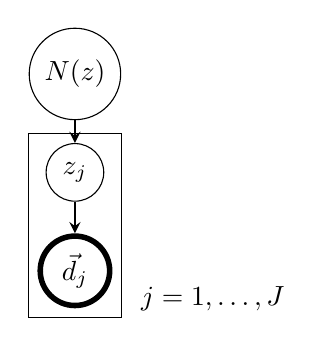
\begin{tikzpicture}[node distance=1cm]

\node (nz) [hyper] {$N(z)$};
\node (z) [param, below of=nz,yshift=-0.25cm] {$z_{j}$};
\node (mags) [data, below of=z,yshift=-0.25cm] {$\vec{d}_{j}$};
\node (survey) [draw=black,fit={(mags.west)(z.north)(mags.south)(mags.east)}] {};
\node [xshift=1.75cm,yshift=0.25cm] at (survey.south) {$j=1,\dots,J$};

\draw [arrow] (nz) -- (z);
\draw [arrow] (z) -- (mags);

\end{tikzpicture}
\caption{This directed acyclic graph illustrates a hierarchical model.}
\label{fig:flow}
\end{center}
\end{figure}

The redshift distribution function $N(z)$ shown in Eq. \ref{eq:distribution} gives the number of galaxies per unit redshift, effectively quantifying evolution in the number of galaxies.  \citep{men13}  According to Eq. \ref{eq:density}, the redshift distribution function is related to the redshift density function $n(z)$, which gives the number of galaxies per unit redshift per unit volume.  The redshift density function provides additional information about cosmology via the rate of expansion over redshift.

\begin{eqnarray}
\label{eq:distribution}
N(z) &=& \frac{dN}{dz}
\end{eqnarray}

\begin{eqnarray}
\label{eq:density}
n(z) &=& \frac{dN}{dz\ d\Omega}
\end{eqnarray}

\clearpage
\subsection{Probabilistic Model}
\label{sec:prob}

We begin by parametrizing $N(z)$ in terms of $\vec{\theta}$, some set of parameters that define the form $N(z)$ may take in whatever basis we choose.  At this point, these hyperparameters are quite general and may represent coefficients in a high-order polynomial as a function of redshift, a set of means and variances defining Gaussians that sum to the desired distribution, a set of histogram heights that describe a binned version of the redshift distribution function, etc.  We define a function $f_{\vec{\theta}}(z)=N(z)$ that transforms these hyperparameters into the redshift distribution function $N(z)$.

We shall denote the size of a given galaxy survey as $J$ galaxies labeled $j$.  The data in this case is a catalog of $J$ sets of photometry $\vec{d}_{j}$ as well as any associated errors on those measurements.  What we wish to estimate is the full posterior probability of the parameters $\vec{\theta}$ given the data $\{\vec{d}_{j}\}_{J}$.  By bayes' Rule, the full posterior may be expressed in terms of the full likelihood by the relation of Eq. \ref{eq:bayes}.  

\begin{eqnarray}
\label{eq:bayes}
p(\vec{\theta}|\{\vec{d}_{j}\}_{J}) &=& \frac{p(\vec{\theta})}{p(\{\vec{d}_{j}\}_{J})}\ p(\{\vec{d}_{j}\}_{J}|\vec{\theta})
\end{eqnarray}

We will have to assume a hyperprior $p(\vec{\theta})$ expressing our beliefs about the distribution of the hyperparameters.  This is a choice we cannot avoid making and one which is often inspired by the results of previous galaxy surveys.  We will, however, probe $\vec{\theta}$ with a quantity proportional to $p(\{\vec{d}_{j}\}_{J}$ because this quantity does not vary with the hyperparameters $\vec{\theta}$ and is generally unknowable.  The last term in this expression is the full likelihood $p(\{\vec{d}_{j}\}_{J}|\vec{\theta})$ of observing the data given the hyperparameters, which may be expanded in terms of a marginalization over the redshifts as parameters, as in Eq. \ref{eq:marginalize}.  

\begin{eqnarray}
\label{eq:marginalize}
p(\{\vec{d}_{j}\}_{J}|\vec{\theta}) &=& \int\ p(\{\vec{d}_{j}\}_{J}|\{z_{j}\}_{J})\ p(\{z_{j}\}_{J}|\vec{\theta})\ d\{z_{j}\}
\end{eqnarray}

We shall make two assumptions of independence in order to make the problem tractable.  First, we take $p(\{\vec{d}_{j}\}_{J}|\{z_{j}\}_{J})$ to be the product of $J$ terms $p(\vec{d}_{j}|z_{j})$, as in Eq. \ref{eq:indiedat}.  This must not be true because of the properties of the survey shared among all observations.  We shall temporarily postpone discussion of the form of the individual likelihoods $p(\vec{d}_{j}|z_{j})$.  

\begin{eqnarray}
\label{eq:indiedat}
p(\{\vec{d}_{j}\}_{J}|\{z_{j}\}_{J}) &=& \prod_{j=1}^{J}\ p(\vec{d}_{j}|z_{j})
\end{eqnarray}

Second, we shall assume the true redshifts $\{z_{j}\}_{J}$ are $J$ independent draws from the general $f_{\vec{\theta}}(z)$.  However, this assumption that the redshift of a galaxy $j$ is independent of the redshift of another galaxy $j'$ must be false because of the shared physical processes of the covariances of $N(z)$.  Additionally, $J$ itself is a Poisson random variable with expected value $J'$.  The combination of these is given by Eq. \ref{eq:indie}  It is important to note that $\int N(z)\ dz$ is not constrained to equal $J'$ but instead $J$, which can be thought of as another parameter.  A detailed discussion of this matter may be found in \citet{for14}.

\begin{eqnarray}
\label{eq:indie}
p(\{z_{j}\}_{J}|\vec{\theta}) &=& \exp\left[-\int\ f_{\vec{\theta}}(z)\ dz\right]\ \prod_{j=1}^{J}\ p(z_{j}|\vec{\theta})
\end{eqnarray}

%The redshift distribution function can be interpreted as being proportional to the likelihood that a random galaxy $j$ has a redshift $z_{j}=z$ where the constant of proportionality is the number $J$ of galaxies in the survey.  Thus the redshift distribution function we aim to estimate may be expressed in terms of the redshift parameter $z$ according to Eq. \ref{eq:params}.  

We may now combine terms into Eq. \ref{eq:posterior}.

\begin{eqnarray}
\label{eq:posterior}
p(\vec{\theta}|\{\vec{d}_{j}\}_{J}) &\propto& p(\vec{\theta})\ \exp\left[-\int\ f_{\vec{\theta}}(z)\ dz\right]\ \prod_{j=1}^{J}\ \int\ p(\vec{d}_{j}|z_{j})\ p(z_{j}|\vec{\theta})\ dz_{j}
\end{eqnarray}

Eq. \ref{eq:posterior} still contains the individual likelihoods $p(\vec{d}_{j}|z_{j})$ unaddressed since Eq. \ref{eq:marginalize} that are this case is inaccessible; it is worth discussing why this is the case.  Both empirical and data-driven methods for obtaining zPDFs effectively assign to each galaxy's photometry $\vec{d}_{j}$ both a redshift $z_{j}$ and some nuisance parameters contained in $\vec{\theta}^{0}$ related to the generative model for photometry from redshifts, encapsulated by $p(z_{j}|\vec{d}_{j},\vec{\theta}^{0})$.  These may include some parameters defining intrinsic galaxy spectra and instrumental effects, for example. (See \citet{ben98} for more detail.)  In the case of estimating $N(z)$ photometrically it is common to use $\vec{\theta}^{0}$ corresponding to $N(z)$ derived from some different, spectroscopically confirmed sample or from a cosmological simulation.  For statistical purposes, we would like any interim prior to be uninformative, but this is rarely achievable.

%If we were to attempt to calculate likelihoods $p(\vec{d}_{j}|z_{j},\vec{\theta}^{0})$, we would be unable to integrate out these nuisance parameters.  (See \citet{hog12} for a comprehensive presentation of the mathematics behind why this is the case.)  However, posteriors $p(z_{j},\vec{\theta}^{0}|\vec{d}_{j})$ could be transformed to zPDFs $p(z_{j}|\vec{d}_{j},\vec{\theta}^{0})$ by integrating $p(z_{j},\vec{\theta}^{0}|\vec{d}_{j})\ p(\vec{\theta}^{0})$ with respect to $\vec{\theta}^{0}$, given the prior  $p(\vec{\theta}^{0})$ of those parameters.  

Instead, we would like to work with posteriors rather than likelihoods in Eq. \ref{eq:marginalize}.  The method outlined here is valid regardless of how the zPDF $p(z_{j}|\vec{d}_{j},\vec{\theta}^{0})$ is calculated so the approach to producing zPDFs will not be discussed; though the matter is outside the scope of this paper, various methods have been presented in the literature. \citep{she11, bal08, car13, car14a}  However, we will need an explicit statement of this interim prior $\vec{\theta}^{0}$ for whatever method is chosen to produce zPDFs.  To perform the necessary transformation from likelihoods to posteriors, we follow the reasoning of \citet{mar15}.  Let us consider the probability of the parameters $z_{j}$ conditioned on the data $\vec{d}_{j}$ and an interim prior $\vec{\theta}^{0}$ and rewrite the problematic likelihood of Eq. \ref{eq:posterior} as Eq. \ref{eq:trick}.  

\begin{eqnarray}
\label{eq:trick}
p(\vec{d}_{j}|z_{j}) &=& p(\vec{d}_{j}|z_{j})\ \frac{p(z_{j}|\vec{d}_{j},\vec{\theta}^{0})}{p(z_{j}|\vec{d}_{j},\vec{\theta}^{0})}
%p(\vec{\theta}|\{\vec{d}_{j}\}_{J}) &=& \frac{p(\vec{\theta})}{p(\{\vec{d}_{j}\}_{J})}\exp[-\int N(z)\ dz]\prod_{j=1}^{J}\int\ p(\vec{d}_{j}|z_{j})\ p(z_{j}|\vec{\theta})\ \frac{p(z_{j}|\vec{d}_{j},\vec{\theta}^{0})}{p(z_{j}|\vec{d}_{j},\vec{\theta}^{0})}\ dz_{j}
\end{eqnarray}

Once the interim prior $\vec{\theta}^{0}$ is explicitly introduced, we may expand the denominator according to Eq. \ref{eq:bayes} to get Eq. \ref{eq:expand}.  We again expand the term $p(\vec{d}_{j}|z_{j},\vec{\theta}^{0})$ to obtain Eq. \ref{eq:indterm}.  Canceling the undesirable likelihood terms $p(\vec{d}_{j}|z_{j})$ and $p(\vec{d}_{j}|\vec{\theta}^{0})$ yields Eq. \ref{eq:cancel}.  We put this all together to get the full posterior Eq. \ref{eq:final}.

\begin{eqnarray}
\label{eq:expand}
p(\vec{d}_{j}|z_{j}) &=& p(\vec{d}_{j}|z_{j})\ p(z_{j}|\vec{d}_{j},\vec{\theta}^{0})\ \frac{p(\vec{d}_{j}|\vec{\theta}^{0})}{p(z_{j}|\vec{\theta}^{0})\ p(\vec{d}_{j}|z_{j},\vec{\theta}^{0})}
%p(\vec{\theta}|\{\vec{d}_{j}\}_{J}) &=& \frac{p(\vec{\theta})}{p(\{\vec{d}_{j}\}_{J})}\exp[-\int N(z)\ dz]\prod_{j=1}^{J}\int\ p(\vec{d}_{j}|z_{j})\ p(z_{j}|\vec{\theta})\ p(z_{j}|\vec{d}_{j},\vec{\theta}^{0})\ \frac{p(\vec{d}_{j}|\vec{\theta}^{0})}{p(\vec{d}_{j}|z_{j},\vec{\theta}^{0})\ p(z_{j}|\vec{\theta}^{0})}\ dz_{j}
\end{eqnarray}

\begin{eqnarray}
\label{eq:indterm}
p(\vec{d}_{j}|z_{j}) &=& p(\vec{d}_{j}|z_{j})\ p(z_{j}|\vec{d}_{j},\vec{\theta}^{0})\ \frac{p(\vec{d}_{j}|\vec{\theta}^{0})}{p(z_{j}|\vec{\theta}^{0})\ p(\vec{d}_{j}|z_{j})\ p(\vec{d}_{j}|\vec{\theta}^{0})}
%p(\vec{\theta}|\{\vec{d}_{j}\}_{J}) &=& \frac{p(\vec{\theta})}{p(\{\vec{d}_{j}\}_{J})}\exp[-\int N(z)\ dz]\prod_{j=1}^{J}\ \int\ p(z_{j}|\vec{d}_{j},\vec{\theta}^{0})\ \frac{p(z_{j}|\vec{\theta})}{p(z_{j}|\vec{\theta}^{0})}\ dz_{j}
\end{eqnarray}

\begin{eqnarray}
\label{eq:cancel}
p(\vec{d}_{j}|z_{j}) &=& \frac{p(z_{j}|\vec{d}_{j},\vec{\theta}^{0})}{p(z_{j}|\vec{\theta}^{0})}
%p(\vec{\theta}|\{\vec{d}_{j}\}_{J}) &=& \frac{p(\vec{\theta})}{p(\{\vec{d}_{j}\}_{J})}\exp[-\int N(z)\ dz]\prod_{j=1}^{J}\ \int\ p(z_{j}|\vec{d}_{j},\vec{\theta}^{0})\ \frac{p(z_{j}|\vec{\theta})}{p(z_{j}|\vec{\theta}^{0})}\ dz_{j}
\end{eqnarray}

\begin{eqnarray}
\label{eq:final}
%p(\vec{\theta}|\{\vec{d}_{j}\}_{J}) &=& \frac{p(\vec{\theta})}{p(\{\vec{d}_{j}\}_{J})}\exp[-\int N(z)\ dz]\prod_{j=1}^{J}\ \int\ p(z_{j}|\vec{d}_{j},\vec{\theta}^{0})\ \frac{p(z_{j}|\vec{\theta})}{p(z_{j}|\vec{\theta}^{0})}\ dz_{j}
p(\vec{\theta}|\{\vec{d}_{j}\}_{J}) &\propto& p(\vec{\theta})\ \exp\left[-\int\ f_{\vec{\theta}}(z)\ dz\right]\ \prod_{j=1}^{J}\ \int\ p(z_{j}|\vec{d}_{j},\vec{\theta}^{0})\ \frac{p(z_{j}|\vec{\theta})}{p(z_{j}|\vec{\theta}^{0})}\ dz_{j}
\end{eqnarray}

The argument of the integral in the posterior of Eq. \ref{eq:final} depends solely on knowable quantities (and those we must assume) and can be calculated for a given set of zPDFs $\{p(z_{j}|\vec{d}_{j},\vec{\theta}^{0})\}_{J}$ and the interim prior $\vec{\theta}^{0}$ upon which their determination was based, noting the relation of Eq. \ref{eq:params}.  Since we cannot know $p(\{\vec{d}_{j}\}_{J})$, we sample the desired distribution $p(\vec{\theta}|\{\vec{d}_{j}\}_{J})$ using Monte Carlo-Markov chain (MCMC) methods.  

\begin{eqnarray}
\label{eq:params}
p(z_{j}|\vec{\theta}) &=& \frac{f_{\vec{\theta}}(z_{j})}{\int\ f_{\vec{\theta}}(z_{j})\ dz_{j}}
\end{eqnarray}

To be clear, the following assumptions must be made in order to apply this method:

\begin{enumerate}
\item Photometric measurements of galaxies are independent Poisson draws from the set of all galaxies such that Eqs. \ref{eq:indiedat} and \ref{eq:indie} hold.
\item We take the individual galaxy zPDFs to be accurate estimates of the posteriors $\{p(z_{j}|\vec{d}_{j})\}_{J}$ and assume we are given the interim prior $\vec{\theta}^{0}$ used to produce them.
\item One must assume a hyperprior $p(\vec{\theta})$ constraining the underlying probability of the variables defining the hyperparameters $\vec{\theta}$.
\end{enumerate}

These assumptions have known limitations.  First, the observations $\{\vec{d}_{j}\}_{J}$ are not a set of independent measurements; they are correlated not only by the conditions of the experiment under which they were made but also by $N(z)$ and other physical processes governing underlying galaxy spectra.  Second, the zPDFs $\{p(z_{j}|\vec{d}_{j},\vec{\theta}^{0})_{J}$ may not be trustworthy; there is not yet agreement on the best technique to obtain zPDFs, and the interim prior $\vec{\theta}^{0}$ may not be appropriate or even known to us as consumers of zPDFs.  Third, the hyperprior $p(\vec{\theta})$ may be quite arbitrary; it may be poorly motivated if the underlying physics is complex.

\clearpage
\section{Experiments}
\label{sec:exp}

We ran several tests of this approach to demonstrate its validity and usage using a procedure outlined in this section.  In Sec. \ref{sec:mock} we describe the method by which sets of simulated zPDFs $\{p(z_{j}|\vec{d}_{j})\}_{J}$ are generated in all test cases.  In Sec. \ref{sec:mcmc} we describe the algorithm used to compute the full posterior distribution $p(\vec{\theta}|\{\vec{d}_{j}\}_{J})$.  In Sec. \ref{sec:diag} we outline the measures used to evaluate the performance of the method, including the competing methods with which our results will be compared.  Then in Sec. \ref{sec:valid} we motivate and present the results of several informative tests.

\clearpage
\subsection{Mock data}
\label{sec:mock}

Data simulation consists of several broad steps described below.  First a true value of $\vec{\theta}$ will be chosen in Sec. \ref{sec:theta}.  Then the true redshifts of all galaxies in the simulated survey will be set in Sec. \ref{sec:z}.  Finally the zPDFs for all surveyed galaxies will be generated in Sec. \ref{sec:d}.

\clearpage
\subsubsection{True redshift distribution}
\label{sec:theta}

The following procedure is executed to generate a true set of parameters $\tilde{\vec{\theta}}$.  First we assume a discretization of redshifts, an underlying redshift density function, a parametrization for $N(z)$, and a target survey size.  Then a true catalog size is chosen.  Finally the true underlying redshift distribution is sampled to obtain the true parameters $\tilde{\vec{\theta}}$.

We consider $K'$ redshift bins $B_{k'}=[z^{B}_{k'-1},z^{B}_{k'}]$ over a range from $z^{B}_{0}=z_{min}$ to $z^{B}_{K'}=z_{max}$.  The widths of the bins are denoted as $\Delta_{k'}\equiv z_{k'}-z_{k'-1}$.

We assume the underlying shape of $N(z)$, defined by some physically-motivated $p^{0}(z)$.  Here we shall set it to a sum of arbitrary Gaussians chosen to impose features on the true $N(z)$.  The underlying $p^{0}(z)$ must be binned down according to the discretization of redshift space chosen.  An example of this binned parametrization of $p(z)$ is shown in Fig. \ref{fig:physPz} and given by Eq. \ref{eq:truepz}.

\begin{eqnarray}
\label{eq:truepz}
p^{0}(z_{k'}) &=& \sum_{c=1}^{5}\bar{z}_{k'}C_{c}\int_{z_{k'}}^{z_{k'+1}} \mathcal{N}(z_{c},\sigma_{c})dz
\end{eqnarray}

\begin{figure}
\label{fig:physPz}
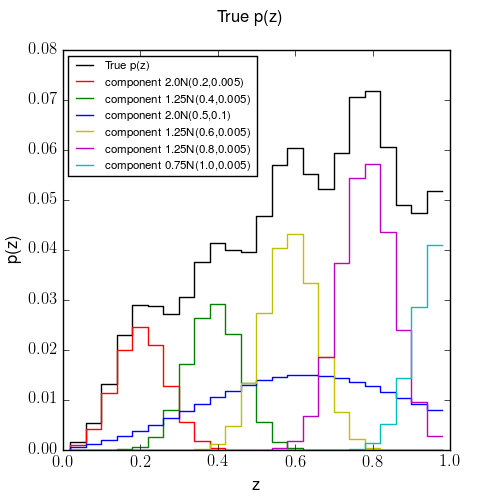
\includegraphics[width=0.5\textwidth]{physPz.png}
\caption{The underlying $p(z)$ is a sum of Gaussians.  Here it is shown for the case of $K'=25$ bins from $z_{0}=0$ to $z_{K'}=1$}
\end{figure}

We shall take $\vec{\theta}$ to be a discretized parametrization of $N(z)$ in log-space, where $\exp[\theta_{k'}]$ is the average value of $N(z)$ over the redshift range of bin $B_{k'}$.   The elements of $\vec{\theta}$ may thus be thought of as histogram heights in a binned version of $\ln N(z)$.  

We choose a target survey size of $J'$ galaxies.  This enables the definition of an underlying $N(z)$  parametrized by $\vec{\theta}'$ defined in terms of the binned parametrization of $p(z)$.  The expected number of galaxies in bin $k'$ is given in Eq. \ref{eq:dparams} (which is an extension of Eq. \ref{eq:params}).  

\begin{eqnarray}
\label{eq:dparams}
B_{k'} &\sim& \frac{\exp[\theta'_{k'}]\Delta_{k'}}{J'}
\end{eqnarray}

We then select the number of galaxies $J$ actually observed in the simulated survey from a Poisson distribution centered around the expected survey size $J'$, as in Eq. \ref{eq:poisson}.  This relates the underlying $p(z)$ to an underlying $N(z)$.

\begin{eqnarray}
\label{eq:poisson}
p(J|J') &=& \frac{J'^{J}\ \exp[-J']}{J!}
\end{eqnarray}

Finally we are ready to set the true values of the parameters comprising $\tilde{\vec{\theta}}$.  Using the probabilities defined by $\vec{\phi}$, we take a sample of $J$ values of $B_{j}$ from the underlying distribution $p(B_{j}|\vec{\theta})$ defined in Eq. \ref{eq:dparams}, giving a set of true redshift bins $\{B_{j}\}_{J}$ for all galaxies $j$, with $J_{k'}$ galaxies falling into bin $k'$.  The log of the resulting proportion of the population $\ln[\frac{J_{k'}}{J}]$ in bin $k'$ is related to the true value $\tilde{\theta}_{k'}$ of the hyperparameters for the binned redshift distribution function given in Eq. \ref{eq:nparams}.  This is precisely the quantity to which we must compare the results of this technique to evaluate its performance.

\begin{eqnarray}
\label{eq:nparams}
B_{j'} &\sim& \left\{\begin{array}{cc}\exp[\tilde{\theta}_{k'}]\ \Delta_{k'}&B_{j'}=B_{k'}\end{array}\right\}
\end{eqnarray}

\clearpage
\subsubsection{True redshifts}
\label{sec:z}

Once the hyperparameters are fixed, we choose the redshift parameters by assigning to each galaxy $j$ a true redshift $z_{j}^{0}$.  These are chosen uniformly from within the bin $B_{j}$ to which it was assigned, according to Eq. \ref{eq:uniform}.  We shall denote the true values of the parameters as $\{z_{j}^{0}\}_{J}$. 

\begin{eqnarray}
\label{eq:uniform}
z_{j}^{0} &\sim& \left\{\begin{array}{cc}\frac{1}{z^{B}_{k'}-z^{B}_{k'-1}} & B_{j} = B_{k'}\\0 & B_{j} \neq B_{k'}\end{array}\right\}
\end{eqnarray}

\clearpage
\subsubsection{Observed zPDFs}
\label{sec:d}

Lastly, we simulate the "observed" zPDFs.  zPDFs taking the form of a Gaussian distribution around some maximum a posteriori redshift are the simplest extension of point estimates with reported error bars.  To simulate the innacuracy in measurements, the true redshift of each galaxy $z_{j}^{0}$ is transformed to a shifted redshift $z_{j}'$.  To simulate the fact that such inaccuracy increases at higher redshift, the $z_{j}'$ are drawn from the Gaussian distribution of Eq. \ref{eq:zshift} with mean of $z_{j}^{0}$ and variance $\delta_{j}\propto(1+z_{j}^{0})^{2}$ given by Eq. \ref{eq:zshift-how}.  

\begin{eqnarray}
\label{eq:zshift}
z_{j}' &\sim& \mathcal{N}(z_{j}^{0},\delta_{j})
\end{eqnarray}

\begin{eqnarray}
\label{eq:zshift-how}
\delta_{j} &=& \bar{\Delta}(1+z^{0}_{j})
\end{eqnarray}

The $J$ continuous zPDFs are then Gaussians given by Eq. \ref{eq:zspread}, where each Gaussian has mean equal to the shifted redshift $z_{j}'$ and variance $\delta_{j}$ to simulate the fact that the imprecision increases with redshift.  We may thus record a "catalog" of data comprised of $J$ sequences $j$ with elements of the form of a pair $(z_{j}',\delta_{j})$ from which binned zPDFs may be constructed for any parametrization of redshift.  

\begin{eqnarray}
\label{eq:zspread}
p(z_{j}|z_{j}') &=& \mathcal{N}(z_{j}',\delta_{j})\ \equiv\ p(z_{j}|\vec{d}_{j})
\end{eqnarray}

To obtain the desired $p(z_{j}|\vec{d}_{j},\vec{\theta}^{0})$, we make use of the interim prior $\vec{\theta}^{0}$ introduced in Eq. \ref{eq:trick} that encodes our beliefs about the way data is produced by way of Eq. \ref{eq:interim}.  The term $\frac{p(z_{j}|\vec{\theta}^{0})}{p(z_{j})}\equiv f_{\vec{\theta}^{0}}(z_{j})$ represents the interim prior we choose when we run the code.

\begin{eqnarray}
\label{eq:interim}
%p(z_{j}|\vec{\theta}^{0}) &=& %\iint\ p(z_{j}|z'_{j})\ p(z'_{j}|z^{0}_{j})\ p(z^{0}_{j}|\vec{\theta}^{0})\ dz'_{j}\ dz^{0}_{j}
p(z_{j}|\vec{d}_{j},\vec{\theta}^{0}) &=& \frac{p(z_{j}|\vec{\theta}^{0})}{p(z_{j})}\ p(z_{j}|\vec{d}_{j})
\end{eqnarray}

The final step in generating zPDFs is to discretize the relation of Eq. \ref{eq:interim}.  In order to accommodate galaxies whose maximal a posteriori redshifts $z_{j}$ are below or above the bounds of the original $K'$ bins, additional bins $\{B_{k^{-}}\}_{K^{-}}$ and $\{B_{k^{+}}\}_{K^{+}}$ may need to be defined.  The new set of $K=K^{-}+K'+K^{+}$ bins $\{B_{k}\}_{K}$ include the original $K'$ bins but add the newly defined bins that share the original width $\bar{\Delta}$ and span the minimal redshift range necessary to include all $z_{j}$ given that constraint, which is bounded by $z_{k^{-}}\equiv z_{0}-\bar{\Delta}[\max_{z_{j}\leq z_{0}}(z_{0}-_{j})]\mod\bar{\Delta}$ and $z_{k^{+}}\equiv z_{K'}+\bar{\Delta}[\max_{z_{j}\geq z_{K'}}(z_{j}-z_{K'})]\mod\bar{\Delta}$.  The discretized posterior $p(B_{k}|\vec{d}_{j})$ for each galaxy is given by Eq. \ref{eq:zdist} in terms of the quantities available in the catalog and normalized to integrate to unity over the redshift range $[z_{k^{-}},z_{k^{+}}]$.  

\begin{eqnarray}
\label{eq:zdist}
p(B_{k}|\vec{d_{j}}) = \frac{\int_{z_{k}}^{z_{k+1}}\ \frac{f_{\vec{\theta}^{0}}(z_{j})}{\sqrt{2\pi\delta_{j}}}\ \exp\left[-\frac{(z'_{j}-z_{j})^{2}}{2\delta_{j}}\right]\ dz_{j}}{\int_{z_{k^{-}}}^{z_{k^{+}}}\ \frac{f_{\vec{\theta}^{0}}(z_{j})}{\sqrt{2\pi\delta_{j}}}\ \exp\left[-\frac{(z'_{j}-z_{j})^{2}}{2\delta_{j}}\right]\ dz_{j}}
\end{eqnarray}

\clearpage
\subsection{Computation}
\label{sec:mcmc}

The form of the full posterior of Eq. \ref{eq:final} must be adapted for the parametrization of redshift space chosen in Sec. \ref{sec:mock}.  Since $p(\{\vec{d}_{j}\}_{J})$ is in general unknown, we will commence working with $\tilde{p}(\vec{\theta}|\{\vec{d}_{j}\}_{J})$, a quantity proportional to the full posterior $p(\vec{\theta}|\{\vec{d}_{j}\}_{J})$, which shall be called the "pseudo-posterior," given in Eq. \ref{eq:discpost}.  We shall work with log probabilities from this point forward for computational efficiency and numerical stability.  A simplified expression for the log of Eq. \ref{eq:discpost} is given in Eq. \ref{eq:logpost}.

\begin{eqnarray}
\label{eq:discpost}
\tilde{p}(\vec{\theta}|\{\vec{d}_{j}\}_{J}) &=& p(\vec{\theta})\ \exp\left[-\sum_{k=1}^{K}\exp[\theta_{k}]\Delta_{k}\right]\ \prod_{j=1}^{J}\ \sum_{k=1}^{K}\ p(B_{k'}|\vec{d}_{j},\theta^{0}_{k})\ \frac{\exp[\theta_{k}]}{\exp[\theta_{k}^{0}]}\ \Delta_{k}
\end{eqnarray}

\begin{eqnarray}
\label{eq:logpost}
\ln[\tilde{p}(\vec{\theta}|\{\vec{d}_{j}\}_{J})] = \ln[p(\vec{\theta})]-\sum_{k=1}^{K}\exp[\theta_{k}]\Delta_{k}+\sum_{j=1}^{J}\ln\left[\sum_{k=1}^{K}\exp\left[\ln[p(B_{k}|\vec{d}_{j},\vec{\theta}^{0})]+\theta_{k}-\theta_{k}^{0}+\ln[\Delta_{k}]\right]\right]
\end{eqnarray}

The Metropolis-Hastings algorithm is applied to sample the full posterior of Eq. \ref{eq:logpost}.  The testing procedure was written in \texttt{Python} and employs the \texttt{emcee} implementation of the algorithm.  \citep{for12}  The input/output format chosen for this work is \texttt{HDF5} because of its efficiency for large amounts of data.

The code takes as input a \texttt{csv} file containing the basis for the parametrization of redshift space, a specification of the interim prior $\vec{\theta}^{0}$, and a catalog of $J$ zPDFs $\{p(B_{j}|\vec{d}_{j},\vec{\theta}^{0})\}_{J}$ in some basis.  The form of the data is a set of $J$ elements each with $K$ values each representing the continuous distribution function (CDF) over the $k$th bin.

The procedure is initialized with a prior distribution $p(\vec{\theta})$ equal to a multivariate normal distribution with mean $\vec{\mu}$ and covariance $\textul{\Sigma}$, the choices of which shall be made to permit draws from this prior distribution to produce shapes similar to that of the true $\tilde{\theta}$.  At each iteration $i$, a proposal distribution $\vec{\theta}^{i}$ generated from this prior distribution and evaluated for acceptance to or rejection from the desired posterior distribution according to the algorithm outlined below.  %Some examples of samples from the initialization value are shown in Fig. \ref{fig:priors}.

%\begin{figure}
%\label{fig:priors}
%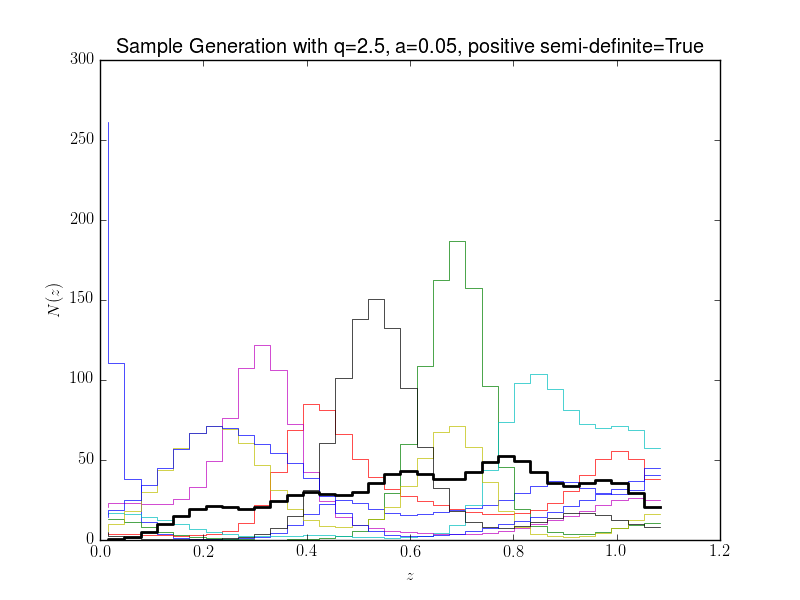
\includegraphics[width=\textwidth]{samples5.png}
%\caption{Several random samples of $\vec{\theta}$ from the distribution of Eq. \ref{eq:covmat} are shown here.  %As $a$ increases, more peaks are permitted and the distribution becomes less smooth.  For a set value of $q$, the amplitude of deviations from the mean decreases with $a$.
%}
%\end{figure}

\begin{enumerate}
\item \label{it:randsamp} Randomly sample the interim prior $p(\vec{\theta})$ to generate a proposal $\vec{\theta}^{i}$.
\item Calculate the log pseudo-posterior as in Eq. \ref{eq:logpost} to produce $\ln\tilde{p}(\vec{\theta}^{i}|\{\vec{d}_{j}\}_{J})$.
\item Calculate $a=\ln\tilde{p}(\vec{\theta}^{i}|\{\vec{d}_{j}\}_{J})-\ln\tilde{p}(\vec{\theta}|\{\vec{d}_{j}\}_{J})$.
\item If $a\geq0$, set and record $\vec{\theta}=\vec{\theta}^{i}$.\\
If $a<0$, select a random number $n$ from the uniform distribution between 0 and 1.
\begin{enumerate}
\item If $n<\exp[a]$, set and record $\vec{\theta}=\vec{\theta}^{i}$.
\end{enumerate}
\item Check if the threshold condition has been achieved; if not, return to Step \ref{it:randsamp}.
\end{enumerate}

Here, the threshold condition is defined in terms of sub-runs of $I_{0}$ accepted samples.  When the variance of the log probabilities is less than the change in median log probability over the sub-run, the burn-in period is considered complete.  When this occurs, an additional number of sub-runs equal to the number $I'$ of sub-runs consumed by the burn-in period are completed such that the total number of accepted samples is $I=2I'$.  

The output of the code is a set of $I$ ordered \texttt{hickle} files (should I use \texttt{FITS}?) enumerated by $\rho$ containing the state information after each sub-run.  The state information includes $\frac{I_{0}}{t}$ actual samples $\vec{\theta}^{i}$ for a pre-specified chain thinning factor and their full posterior probabilities $p(\vec{\theta}^{i}|\{\vec{d}_{j}\}_{J})$ as well as the autocorrelation times and acceptance fractions calculated for each element of $\vec{\theta}$ over the entire sub-run.  These two summary statistics are described in Sec. \ref{sec:diag}, along with the proper use of the other outputs in interpreting the results of the code.

\clearpage
\subsection{Diagnostics}
\label{sec:diag}

The results of the computation described in Sec. \ref{sec:mcmc} are evaluated on the basis of four diagnostics measures, briefly described below.  See \citet{for12} for a more complete exploration of these metrics.  The tests conducted here are also compared to the results one would obtain from alternative methods found in the literature, namely the approach of \citet{she11}, which is outlined in \ref{sec:sheldon}

\clearpage
\subsubsection{Autocorrelation Time}
\label{sec:acorr}

The autocorrelation time is effectively a measure of the convergence rate of the method and can be described as the expected number of iterations necessary to accept a sample independent of the current sample.  A sampler that converges faster will have a smaller autocorrelation time, and smaller autocorrelation times are preferable because it means fewer iterations are wasted on non-independent samples when independent samples are desired.  Typically, the autocorrelation time decreases with successive iterations through a burn-in phase before leveling out.

\clearpage
\subsubsection{Acceptance Fraction}
\label{sec:afrac}

Though there is no hard rule for the optimal acceptance fraction for a sampler, we would like it to be high enough that we accept a fair number of samples but low enough that the samples do approach a single distribution.  Commonly accepted goals tend to be between 0.2 and 0.5.  Typically, the acceptance fraction is high during the burn-in phase until some independence from the initial values is achieved, after which it levels out.

\clearpage
\subsubsection{Probability Evolution}
\label{sec:probs}

In order to evaluate the duration of the burn-in phase, it can be helpful to examine the evolution of the posterior probability of each accepted set of parameters.  Though the probability associated with the initial values will likely be quite low, the probability should improve for subsequent accepted parameter values.  As with the diagnostics of Secs. \ref{sec:afrac} and \ref{sec:probs}, the posterior probability of samples will asymptotically approach some more favorable value with more iterations.  The burn-in phase may be identified as the number of iterations necessary before the probabilities are sufficiently close to the value at which they level out.  Samples accepted during the burn-in phase are typically discounted from analysis.

\clearpage
\subsubsection{Parameter Evolution}
\label{sec:params}

An intuitive diagnostic used here is the evolution of the parameter values themselves.  We would like to see each walker move throughout parameter space near the true value rather than remaining stationary or in some small region corresponding to some local maximum of probability that may not be near the true value.  We can visually inspect the parameter values each walker takes over successive iterations to ensure that the walkers are not being caught in small regions of parameter space far from the true parameter values.

\clearpage
\subsubsection{Parameter Values}
\label{sec:samps}

Sampled values of the vector of parameters are also visually inspected for goodness of fit.  If samples are near the true value, the sampler is performing well.  This can also be a good test of the appropriateness of the prior distribution; if the variance of the prior is too restrictive, the walkers will not be able to sample parameter values far from their initialization.  

\clearpage
\subsubsection{Competing Methods}
\label{sec:sheldon}

It is desirable to compare the result of this method to what would have been obtained by two popular methods used in the literature.   The first, hereafter referred to as stacking, directly calculates the posterior for the entire dataset using the posteriors for each galaxy according to Eq. \ref{eq:stack}.  \citep{lim08}  It must be noted here that Eq. \ref{eq:stack} is not mathematically valid.  (See \citet{hog12} for details.)  

\begin{eqnarray}
\label{eq:stack}
\exp[\theta_{k}]\Delta_{k} &=& \sum_{j=1}^{J}\ p(B_{k}|\vec{d}_{j},\vec{\theta}^{0})
\end{eqnarray}

The second method, hereafter referred to as point estimation, converts the individual galaxy posteriors $p(B_{k}|\vec{d}_{j},\vec{\theta}^{0})$ into delta functions at the redshift bin of maximum a posteriori (MAP) probability according to Eq. \ref{eq:map}, or at the redshift bin corresponding to the expected value of Eq. \ref{eq:expval}, before applying Eq. \ref{eq:stack}.  These two methods have been compared to one another by \citet{hil11} and \citet{ben12}.

\begin{eqnarray}
\label{eq:map}
p(B_{k}|\vec{d}_{j},\vec{\theta}^{0}) &=& \left\{\begin{array}{cc}1&argmax_{k}(p(B_{k}|\vec{d}_{j},\vec{\theta}^{0}))\\0&else\end{array}\right\}
\end{eqnarray}

\begin{eqnarray}
\label{eq:expval}
p(B_{k}|\vec{d}_{j},\vec{\theta}^{0}) &=& \left\{\begin{array}{cc}1&\int_{0}^{K} \bar{z}_{k}\ p(B_{k}|\vec{d}_{j},\vec{\theta}^{0}) dk\\0&else\end{array}\right\}
\end{eqnarray}

It is also valuable to verify that the posterior is maximized for the true $N(z)$ that generated a particular set of simulated data and to check the degree to which the samples are unbiased.

\clearpage
\subsubsection{Summary Statistics}
\label{sec:stats}

Beyond visual inspection of samples, we calculate summary statistics to quantitatively compare different estimators' appropriateness for the data.  Three goodness of fit measures of parameter samples $\vec{\theta}^{i}$  have been considered here.  

The likelihood ratio comparing the sampler to competing methods may be calculated for a sample $\vec{\theta}^{i}$ as in Eq. \ref{eq:llr}.  Values of $A$ greater than 0 indicate the sampler fits the data better than the competing method.  The log posterior probabilities of Sec. \ref{sec:probs} are used to obtain the log likelihoods via Eq. \ref{eq:logpost} and the sample values themselves are used to calculate the prior probability term according to Eq. \ref{eq:llr-how}.

\begin{eqnarray}
\label{eq:llr}
A(\vec{\theta}^{i}) &=& -2\ln[\tilde{p}(\{\vec{d}_{j}\}_{J}|\vec{\theta}_{test})]+2\ln[\tilde{p}(\{\vec{d}_{j}\}_{J}|\vec{\theta}^{i})]
\end{eqnarray}

\begin{eqnarray}
\label{eq:llr-how}
\ln[\tilde{p}(\{\vec{d}_{j}\}_{J}|\vec{\theta})] &=& \ln[\tilde{p}(\vec{\theta}|\{\vec{d}_{j}\}_{J})]-\ln[p(\vec{\theta})]
\end{eqnarray}

The mean squared error of samples relative to the true value may also be calculated.  The reported variance $\sigma^{2}$ and $\chi^{2}$ statistic are both calculated for the accepted samples and for the competing methods.

\clearpage
\section{Validation Tests}
\label{sec:valid}

The code was tested on several simulated datasets.  The fiducial experiment of Sec. \ref{sec:null} was generated by code following the procedure given in Sec. \ref{sec:mock}.  Four other cases varied the shapes of the zPDFs (Secs. \ref{sec:noisy} and \ref{sec:multi}), the underlying $N(z)$ (Sec. \ref{sec:fake}), and the interim prior $\vec{\theta}^{0}$ (Sec. \ref{sec:badprior}).  

\clearpage
\subsection{Fiducial Case}
\label{sec:null}

In order to simulate data in the realistic case, we select set a true, physically motivated redshift probability distribution $p^{0}(z|\vec{\theta})$, where $p(z|\vec{\theta})$ corresponds to $\exp[\vec{\theta}]$ for $J=1$.  The instance of $p^{0}(z)$ here is given by Eq. \ref{eq:truepz}, where the constant $C_{c}$ indicates the relative amplitude of the Gaussian component centered at $z_{c}$ with variance $\sigma_{c}^{2}$.  %The linear function is evaluated at the centers of the bins $\bar{z}_{k}=(z_{k+1}-z_{k})/2$ and is included to ensure that $\lim_{z\to0}N(z)=0$.  
The construction of this probability density is illustrated in Fig. \ref{fig:physPz}. 

As in Sec. \ref{sec:theta}, the number of galaxies in the survey $J$ is taken as a random draw from a Poisson distribution centered at $J'=100$.  Taking $p^{0}(z_{k})$ as the probability that galaxy $j$ has a true redshift within bin $B_{k}$, we draw true redshift bins $\{B_{j}\}_{J}$ for all $J$ galaxies in the survey.  The resulting $J_{k}$ define the true value of the parameters $\vec{\tilde{\theta}}$ according to Eq. \ref{eq:sums}.   Fig. \ref{fig:nulltrueNz} shows the true value of $N(z)$ for the fiducial case.

\begin{eqnarray}
\label{eq:sums}
\tilde{\theta}_{k} &=& \ln\left[\frac{J_{k}}{\Delta_{k}}\right]
\end{eqnarray}

\begin{figure}
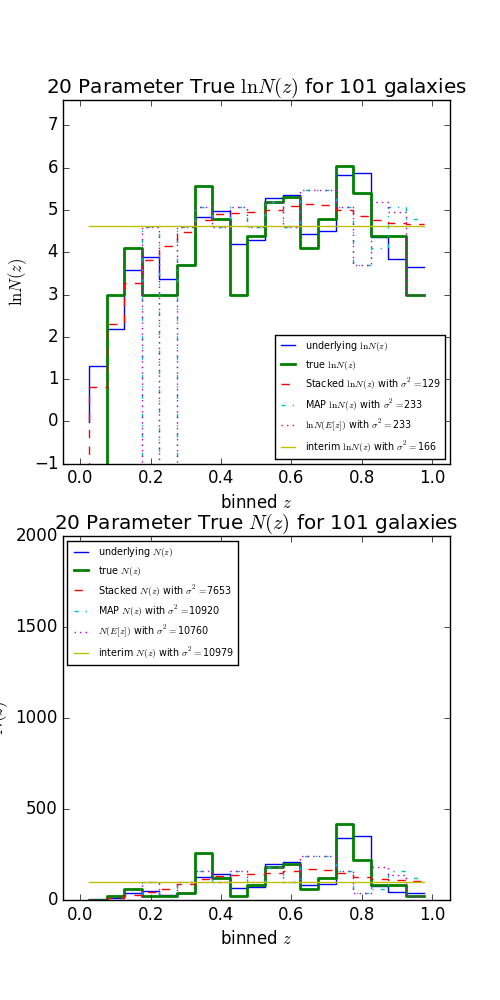
\includegraphics[width=0.5\textwidth]{null/trueNz.png}
\caption{The true value of $N(z)$ in the case of galaxies drawn from the probability distribution of Fig. \ref{fig:physPz}.}
\label{fig:nulltrueNz}
\end{figure}

True redshifts $z^{0}_{j}$ are taken as draws from a uniform distribution within bin $B_{j}$.  The interim prior (discussed in Sec. \ref{sec:d}) used in the fiducial case is a flat $N(z)$ normalized to $J$ galaxies.  The expected and MAP values of redshift of the Gaussian defining the individual posterior, as well as the probability distributions themselves, are plotted against the true redshift in Fig. \ref{fig:realcat}.  The mock data generation procedure of Sec. \ref{sec:fake} is used in this test; samples of some zPDFs used are shown in Fig. \ref{fig:nullpzs}.

\begin{figure}
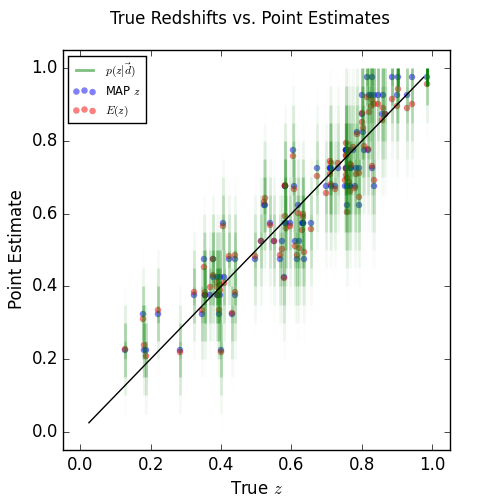
\includegraphics[width=0.5\textwidth]{null/truevmap.png}
\caption{This plot shows the relationship between the true redshift shared by all galaxies in this survey and the redshift at which the posterior is maximized for each galaxy.}
\label{fig:realcat}
\end{figure}

\begin{figure}
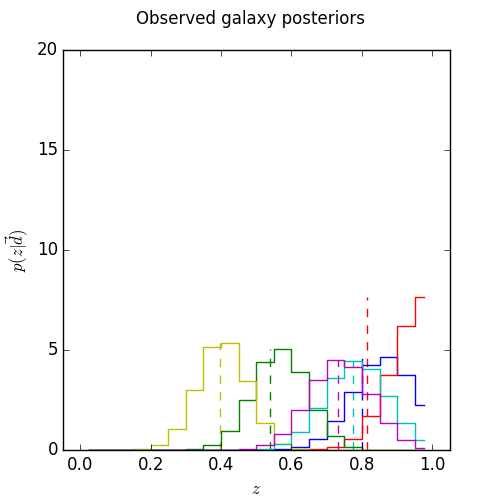
\includegraphics[width=0.5\textwidth]{null/samplepzs.png}
\caption{Unimodal, noiseless zPDFs are used in this test.}
\label{fig:nullpzs}
\end{figure}

We choose an interim prior equal to a multivariate normal distribution with mean satisfying $\vec{\theta}'$ and covariance $\textul{\Sigma}$ given by Eq. \ref{eq:covmat}.  The mean chosen here is that of a flat distribution for the expected number of galaxies in the survey $J'$.  The constants $q$, $a$, and $e$ are small numbers chosen to permit draws from the distribution in question to reproduce shapes similar to that of the true parameters $\vec{\tilde{\theta}}$.  Samples from this prior are shown in Fig. \ref{fig:realprior}.  The calculation is initialized with $20$ walkers each with a value chosen from a Gaussian distribution around a sample of the prior.  The initial values of the walkers are shown in Fig. \ref{fig:realival}.

\begin{eqnarray}
\label{eq:covmat}
\theta'_{k} &=& \ln[J']-\ln[K]-\ln[\Delta_{k}]\\
\Sigma_{kk'} &=& q\exp\left[-\frac{a(k-k')^{2}}{2}\right]+e
\end{eqnarray}

\begin{figure}
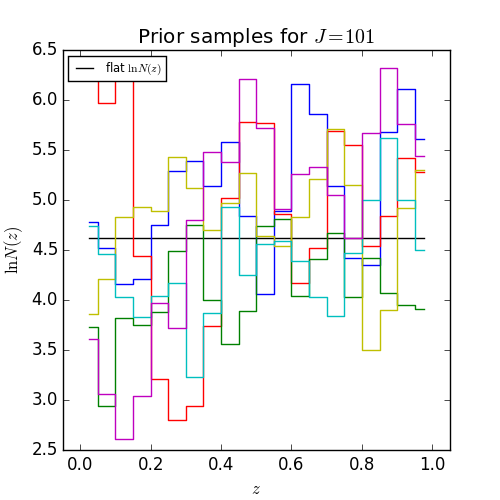
\includegraphics[width=0.5\textwidth]{null/priorsamps.png}
\caption{Examples of draws from the prior of the realistic model.}
\label{fig:realprior}
\end{figure}

\begin{figure}
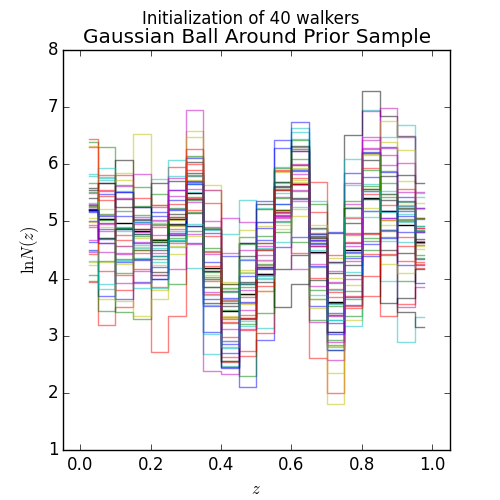
\includegraphics[width=0.5\textwidth]{null/initializations.png}
\caption{The initial values of the walkers are shown here.}
\label{fig:realival}
\end{figure}

The sampler performs well according to the diagnostics discussed in Sec. \ref{sec:diag}, the results of which are shown in Figs. \ref{fig:realacor}, \ref{fig:realfrac}, \ref{fig:realprob}, and \ref{fig:realparam}.  

\begin{figure}
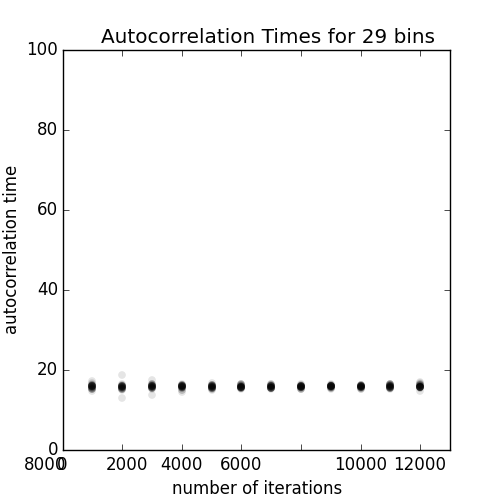
\includegraphics[width=0.5\textwidth]{times-real.png}
\caption{The autocorrelation times are low, indicating fast convergence of the sampler over all parameters.}
\label{fig:realacor}
\end{figure}

\begin{figure}
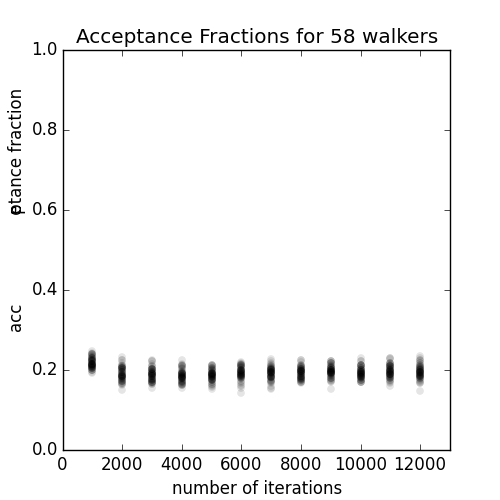
\includegraphics[width=0.5\textwidth]{fracs-real.png}
\caption{The acceptance fractions are reasonable and decrease after the burn-in period.}
\label{fig:realfrac}
\end{figure}

\begin{figure}
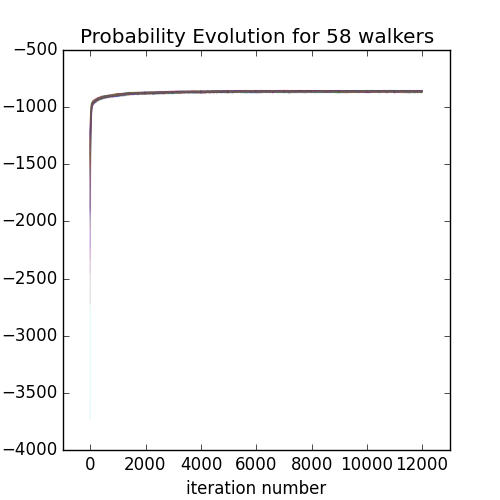
\includegraphics[width=0.5\textwidth]{probs-real.png}
\caption{This plot shows the log probabilities of walkers as a function of iteration number for a number of iterations equal to twice the burn-in period.  One can see that the log posterior probabilities are much greater for the samples than for the alternative methods.}
\label{fig:realprob}
\end{figure}

\begin{figure}
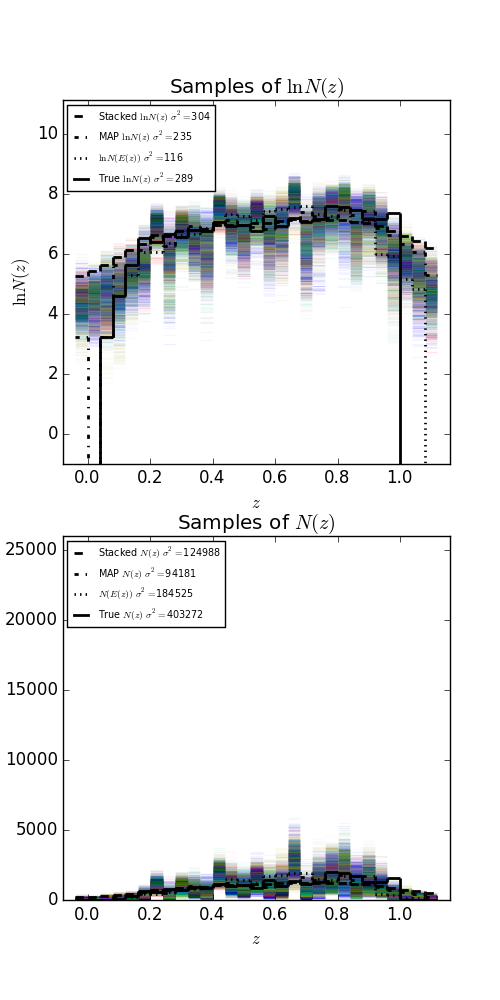
\includegraphics[width=0.5\textwidth]{samps-real.png}
\caption{The results of the simulation may be seen here.  The three statistics considered indicate a different ordering of performance of the estimators.}
\label{fig:realparam}
\end{figure}

\clearpage
\subsection{Noisy zPDFs}
\label{sec:noisy}

In this test, we aim to simulate more realistic zPDFs by modifying the procedure of Sec. \ref{sec:d} to introduce imprecision that increases with true redshift.  

The true redshift distribution is identical to that of \ref{sec:null} (Fig. \ref{fig:nulltrueNz}), as is the method for assigning true redshifts to galaxies.  The zPDFs are still Gaussians but with variances $\delta'_{j}$ that are themselves drawn from a Gaussian of mean $\delta_{j}$ and variance $\delta_{j}^{2}$, transforming Eq. \ref{zshift-how} into Eq. \ref{eq:znoise-how} and Eq. \ref{eq:zspread} into Eq. \ref{eq:znoise}.  Fig. \ref{fig:noisycat} shows the MAP and expected values of redshift, as well as the zPDFs, as a function of the true redshifts.  Fig. \ref{fig:samplepzs} shows a few random zPDFs generated by this procedure.

\begin{eqnarray}
\label{eq:znoise-how}
\delta'_{j} &\sim& \mathcal{N}(\delta_{j},\delta^{2}_{j})
\end{eqnarray}

\begin{eqnarray}
\label{eq:znoise}
p(z_{j}|z'_{j}) &=& \mathcal{N}(z'_{j},\delta'_{j})
\end{eqnarray}

\begin{figure}
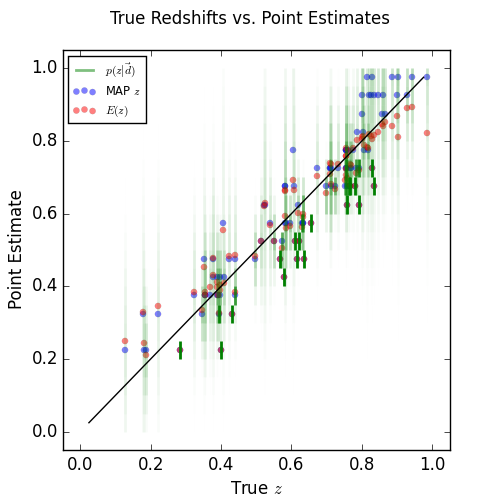
\includegraphics[width=0.5\textwidth]{sigma/truevmap.png}
\caption{This plot shows the relationship between the true redshift shared by all galaxies in this survey and the redshift at which the posterior is maximized for each galaxy.}
\label{fig:noisycat}
\end{figure}

\begin{figure}
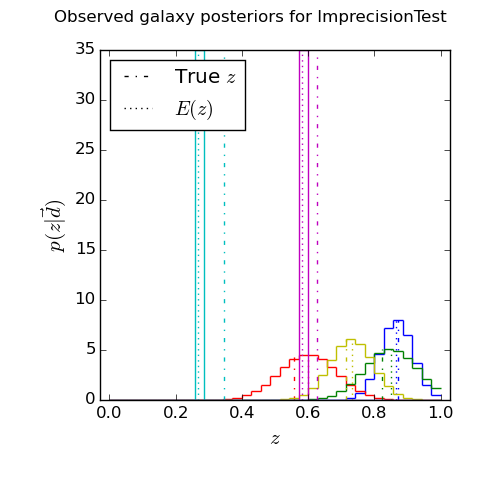
\includegraphics[width=0.5\textwidth]{sigma/samplepzs.png}
\caption{Unimodal, noisy zPDFs are used in this test.  Noise is introduced in the form of variances that are Gaussian random variables rather than fixed values tied to the true redshift.}
\label{fig:noisypzs}
\end{figure}

The sampler is initialized as in Sec. \ref{sec:null}.

%\begin{figure}
%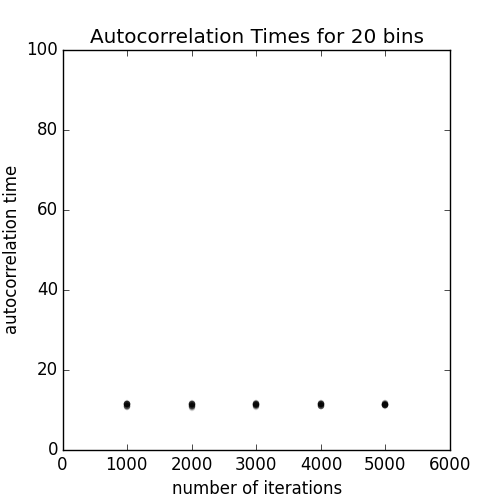
\includegraphics[width=0.5\textwidth]{sigma/times.png}
%\caption{The autocorrelation times are low, indicating fast convergence of the sampler over all parameters.}
%\label{fig:noisyacor}
%\end{figure}
%
%\begin{figure}
%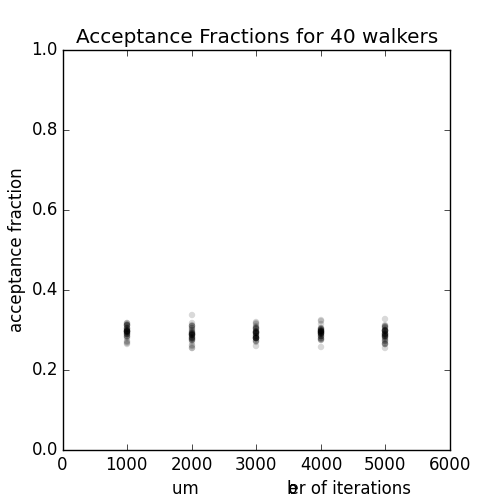
\includegraphics[width=0.5\textwidth]{sigma/fracs.png}
%\caption{The acceptance fractions are reasonable and decrease after the burn-in period.}
%\label{fig:noisyfrac}
%\end{figure}
%
%\begin{figure}
%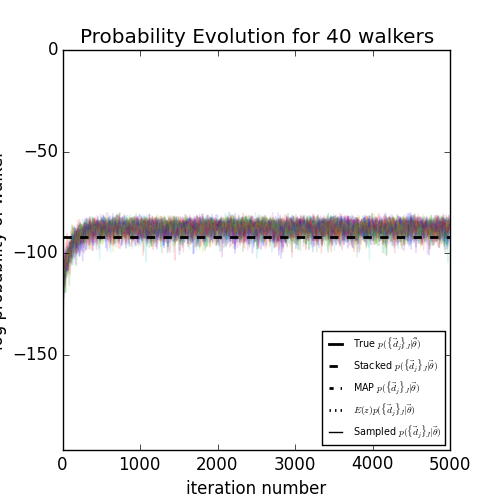
\includegraphics[width=0.5\textwidth]{sigma/probs.png}
%\caption{This plot shows the log probabilities of walkers as a function of iteration number for a number of iterations equal to twice the burn-in period.  One can see that the log posterior probabilities are much greater for the samples than for the alternative methods.}
%\label{fig:noisyprob}
%\end{figure}
%
%\begin{figure}
%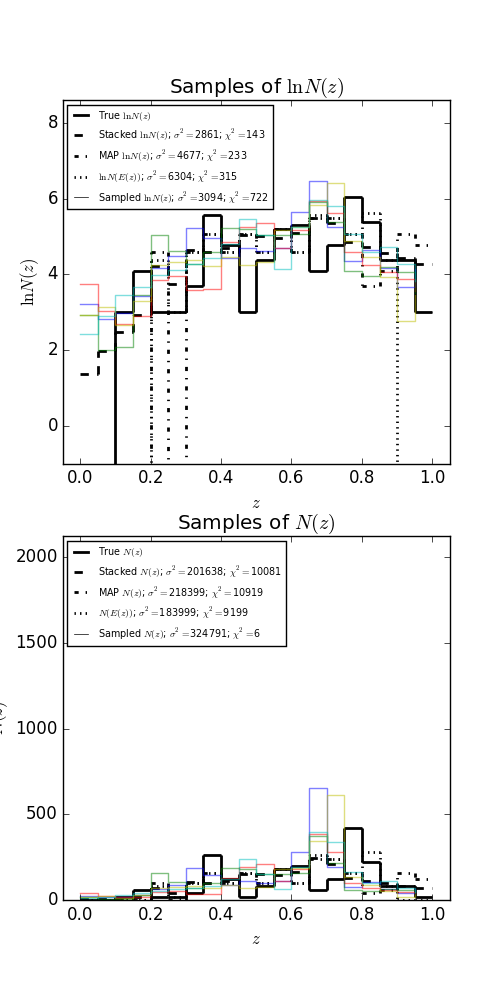
\includegraphics[width=0.5\textwidth]{sigma/samps.png}
%\caption{The results of the simulation may be seen here.  The three statistics considered indicate a different ordering of performance of the estimators.}
%\label{fig:noisyparam}
%\end{figure}

\clearpage
\subsection{Multimodal zPDFs}
\label{sec:multi}

In this test, we aim to simulate more realistic zPDFs by modifying the procedure of Sec. \ref{sec:d} to introduce inaccuracy that causes catastrophic photo-z errors.  Catastrophic photo-z errors arise from a degeneracy in the space of galaxy SEDs and redshifts, wherein a galaxy of one type at one redshift has photometry indistinguishable from a galaxy of another type at another redshift.  To simulate this case, multimodal zPDFs will be considered.

The true $N(z)$ is generated the same way as in Sec. \ref{sec:null} (Fig. \ref{fig:nulltrueNz}).  However, the zPDFs are sums of Gaussians of the form of those tested in Sec. \ref{sec:noisy}.  Each galaxy is first assigned a number $R_{j}$ of Gaussian elements to be summed, chosen randomly from $1,\dots,K$ where $K$ is the dimensionality of $\vec{\theta}$.  The true redshift of each galaxy $z_{j}^{0}$ is transformed to $R_{j}$ shifted redshifts $z^{r_{j}}_{j}$ for $r_{j}=1,\dots,R_{j}$, transforming Eq. \ref{eq:zshift} into Eq. \ref{eq:zmany-each}.  The standard deviations of the Gaussian components follows Eq. \ref{eq:zmany-how}, analogous to Eq. \ref{eq:znoise-how}.  Thus the zPDFs take the form of Eq. \ref{eq:zmany}.  Fig. \ref{fig:multicat} shows the MAP and expected values of redshift as well as the zPDFs as a function of the true redshift.  Some examples of the multimodal zPDFs are shown in Fig. \ref{fig:multipzs}.

\begin{eqnarray}
\label{eq:zmany-each}
z^{r_{j}}_{j} &\sim& \mathcal{N}(z_{j}^{0},\delta_{j})
\end{eqnarray}

\begin{eqnarray}
\label{eq:zmany-how}
\delta^{r_{j}}_{j} &\sim& \mathcal{N}(\delta_{j},\delta^{2}_{j})
\end{eqnarray}

\begin{eqnarray}
\label{eq:zmany}
p(z_{j}|\{z^{r_{j}}_{j}\}_{R_{j}}) &=& \sum_{r_{j}=0}^{R_{j}}\ \mathcal{N}(z^{r_{j}}_{j},\delta^{r_{j}}_{j})
\end{eqnarray}

\begin{figure}
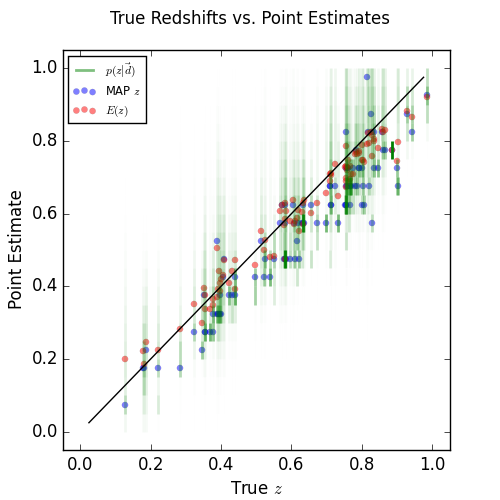
\includegraphics[width=0.5\textwidth]{multi/truevmap.png}
\caption{This plot shows the relationship between the true redshift shared by all galaxies in this survey and the redshift at which the posterior is maximized for each galaxy.}
\label{fig:multicat}
\end{figure}

\begin{figure}
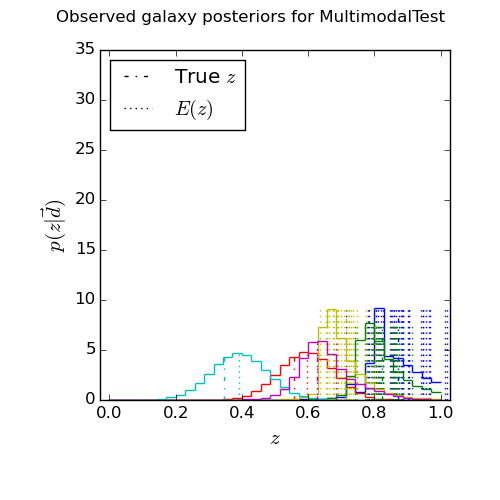
\includegraphics[width=0.5\textwidth]{multi/samplepzs.png}
\caption{Multimodal, noisy zPDFs are used in this test.  Noise is introduced in the form of variances that are Gaussian random variables rather than fixed values tied to the true redshift.}
\label{fig:multipzs}
\end{figure}

The sampler is initialized as in Sec. \ref{sec:null}.

%\begin{figure}
%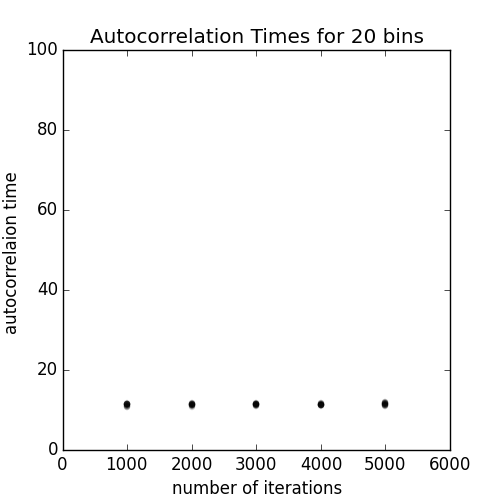
\includegraphics[width=0.5\textwidth]{multi/times.png}
%\caption{The autocorrelation times are low, indicating fast convergence of the sampler over all parameters.}
%\label{fig:multiacor}
%\end{figure}
%
%\begin{figure}
%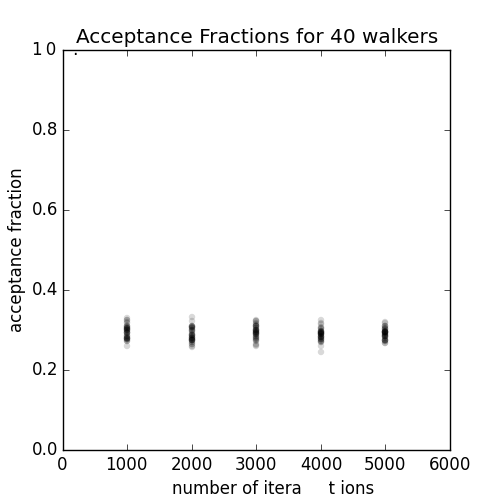
\includegraphics[width=0.5\textwidth]{multi/fracs.png}
%\caption{The acceptance fractions are reasonable and decrease after the burn-in period.}
%\label{fig:multifrac}
%\end{figure}
%
%\begin{figure}
%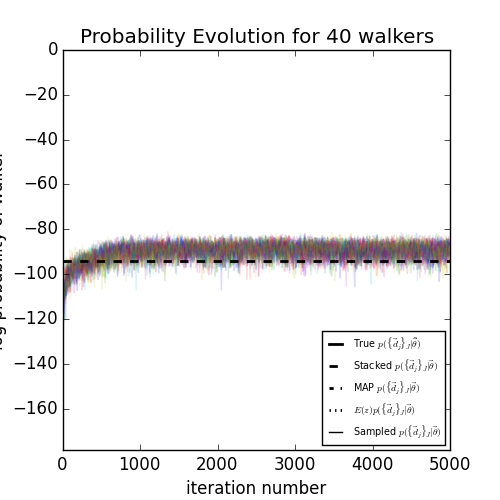
\includegraphics[width=0.5\textwidth]{multi/probs.png}
%\caption{This plot shows the log probabilities of walkers as a function of iteration number for a number of iterations equal to twice the burn-in period.  One can see that the log posterior probabilities are much greater for the samples than for the alternative methods.}
%\label{fig:multiprob}
%\end{figure}
%
%\begin{figure}
%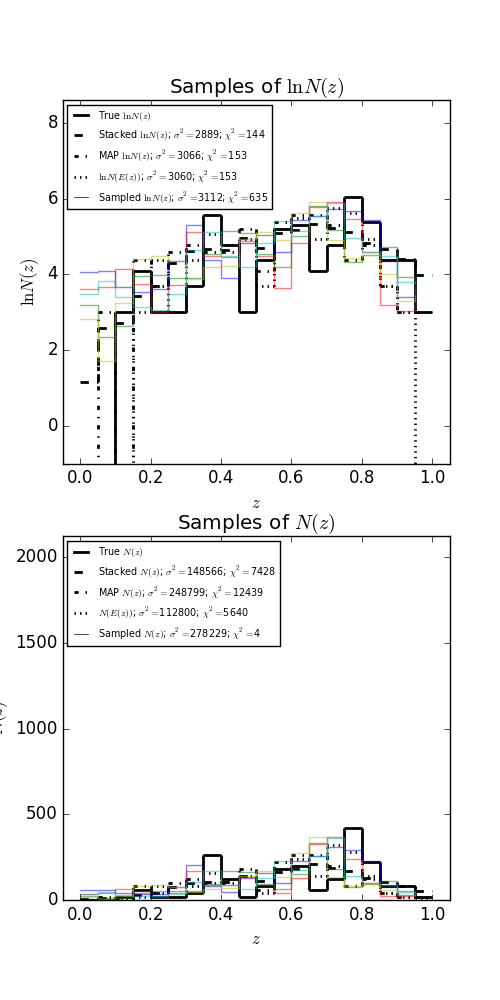
\includegraphics[width=0.5\textwidth]{multi/samps.png}
%\caption{The results of the simulation may be seen here.  The three statistics considered indicate a different ordering of performance of the estimators.}
%\label{fig:multiparam}
%\end{figure}

\clearpage
\subsection{Toy Model $N(z)$}
\label{sec:fake}

We test the sampler in a case of a highly unrealistic but strongly featured underlying $N(z)$.  This is done to show that the sampler works even in extreme conditions.

Here we choose a delta function for the underlying $N(z)$ in which all galaxies have the same true redshift, corresponding to an underlying hyperparameter $\vec{\theta}'$ given by Eq. \ref{eq:faketheta}.  Furthermore, for simplicity, we give all galaxies a single true redshift $z_{j}^{0}=\tilde{z}$ equal to the midpoint of bin $B_{\tilde{k}}$ where $\tilde{k}$ denotes the bin in which $N(z)$ is nonzero.  Only unimodal, noiseless zPDF shapes are considered in this test, as shown in Fig. \ref{fig:toypzs}.  Fig. \ref{fig:toycat} shows the spread in maximum a posteriori values versus the true redshifts for this case.

\begin{eqnarray}
\label{eq:faketheta}
\exp[\theta_{k}'] &=& \left\{\begin{array}{cc}0&k\neq\tilde{k}\\ \frac{J'}{\bar{\Delta}}&k=\tilde{k}\end{array}\right\}
\end{eqnarray}

\begin{figure}
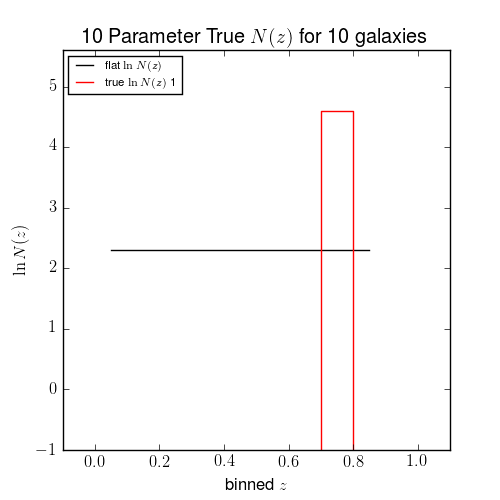
\includegraphics[width=0.5\textwidth]{toy/trueNz.png}
\caption{The true value of $N(z)$ in the test case of all galaxies having the same redshift, compared with a flat $N(z)$ distribution.}
\label{fig:deltatrueNz}
\end{figure}

\begin{figure}
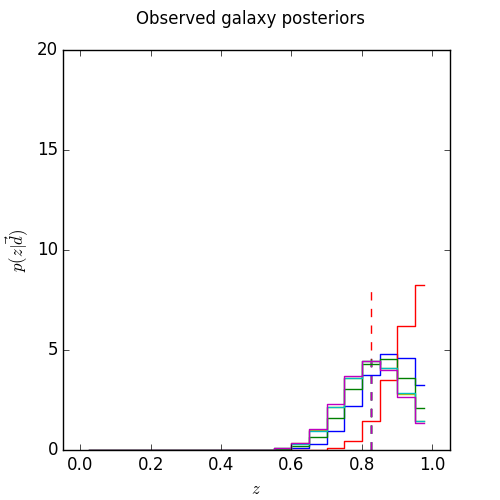
\includegraphics[width=0.5\textwidth]{toy/samplepzs.png}
\caption{Unimodal, noiseless zPDFs are used in this test.}
\label{fig:toypzs}
\end{figure}

\begin{figure}
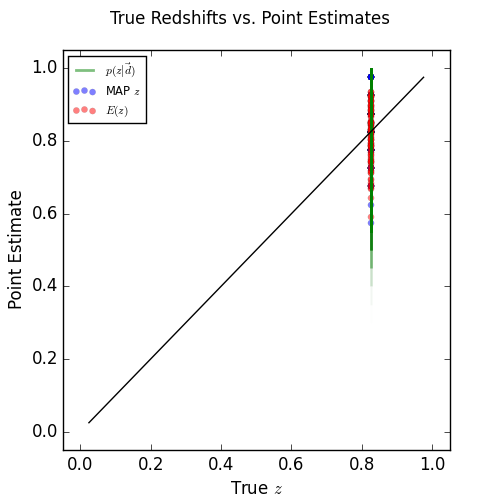
\includegraphics[width=0.5\textwidth]{toy/truevmap.png}
\caption{This plot shows the relationship between the true redshift shared by all galaxies in this survey and the mean redshift of the bin in which the posterior is maximized for each galaxy for each set of mock data tested.}
\label{fig:toycat}
\end{figure}

We initialize the sampler as in Sec. \ref{sec:null} with the same prior.

%\begin{figure}
%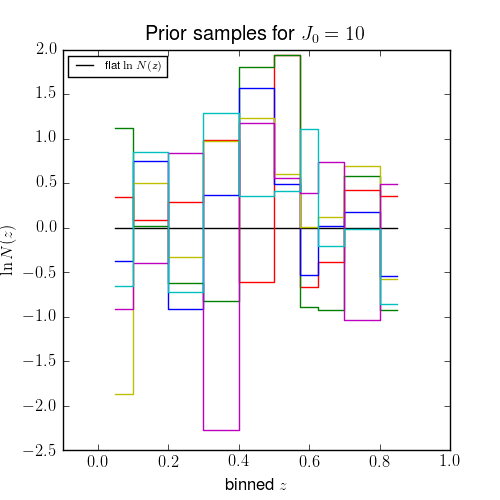
\includegraphics[width=0.5\textwidth]{toy/priorsamps.png}
%\caption{Examples of draws from the prior of the toy model.}
%\label{fig:fakeprior}
%\end{figure}
%
%\begin{figure}
%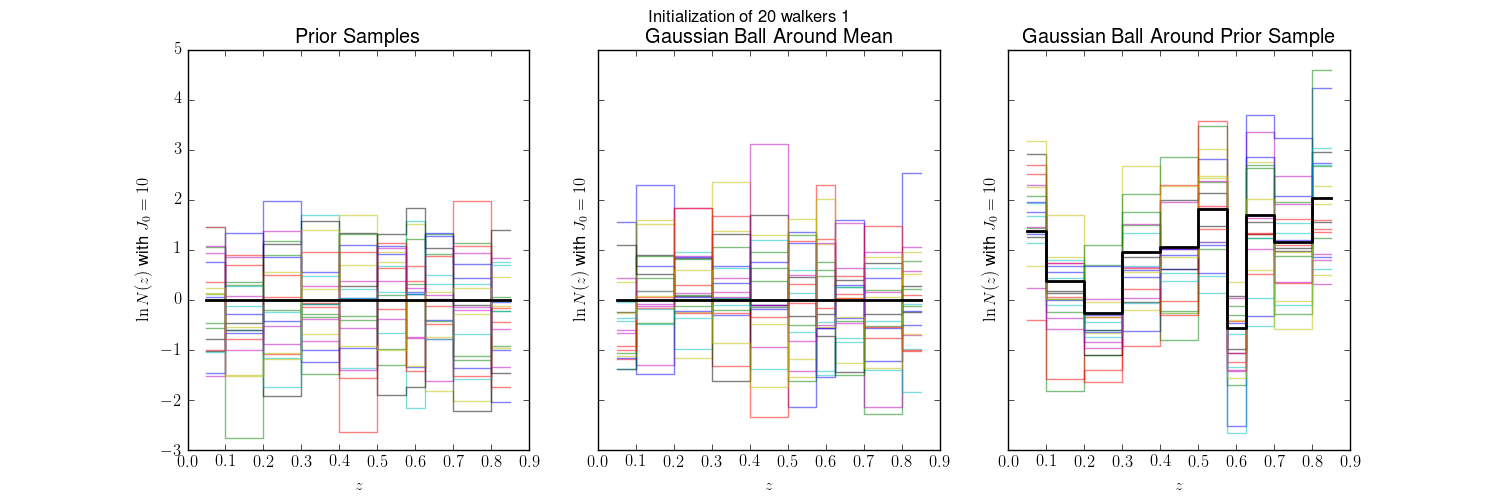
\includegraphics[width=0.5\textwidth]{toy/initializations.png}
%\caption{The initial values of the walkers are samples from a Gaussian ball around a sample from the prior.}
%\label{fig:fakeival}
%\end{figure}

The diagnostics of Sec. \ref{sec:diag} are evaluated and plotted as Figs. \ref{fig:dumbestacor}, \ref{fig:dumbestfrac}, \ref{fig:dumbestprob}, and \ref{fig:dumbestparam} for this test and indicate good convergence and trustworthy samples that outperform the stacked estimator.

\begin{figure}
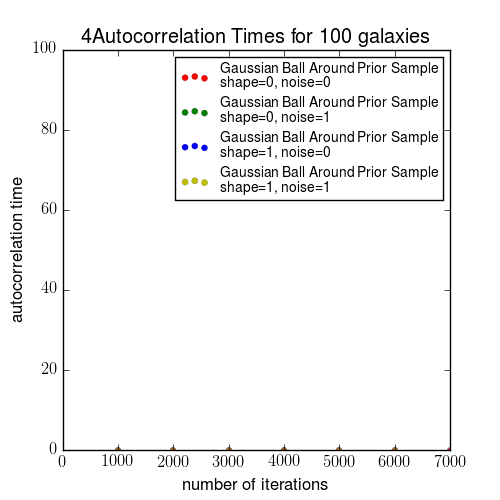
\includegraphics[width=0.5\textwidth]{times-toy.png}
\caption{The autocorrelation times are low, indicating fast convergence of the sampler over all parameters.}
\label{fig:dumbestacor}
\end{figure}

\begin{figure}
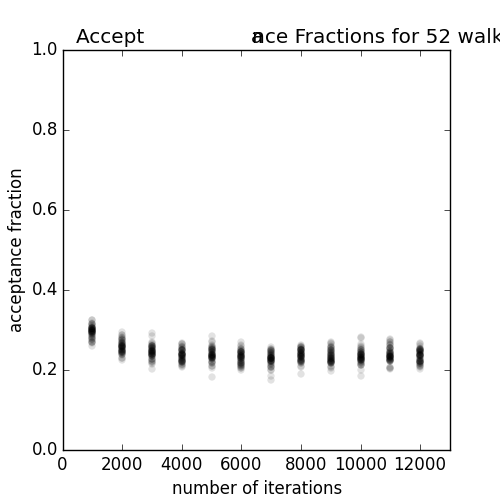
\includegraphics[width=0.5\textwidth]{fracs-toy.png}
\caption{The acceptance fractions are reasonable and decrease after the burn-in period.}
\label{fig:dumbestfrac}
\end{figure}

\begin{figure}
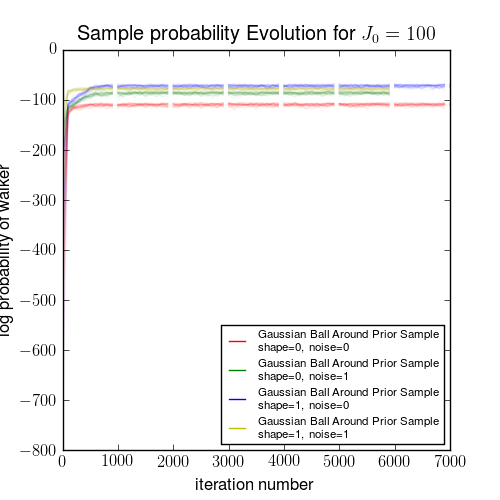
\includegraphics[width=0.5\textwidth]{probs-toy.png}
\caption{This plot shows the log probabilities of walkers as a function of iteration number for a number of iterations equal to twice the burn-in period.}
\label{fig:dumbestprob}
\end{figure}

\begin{figure}
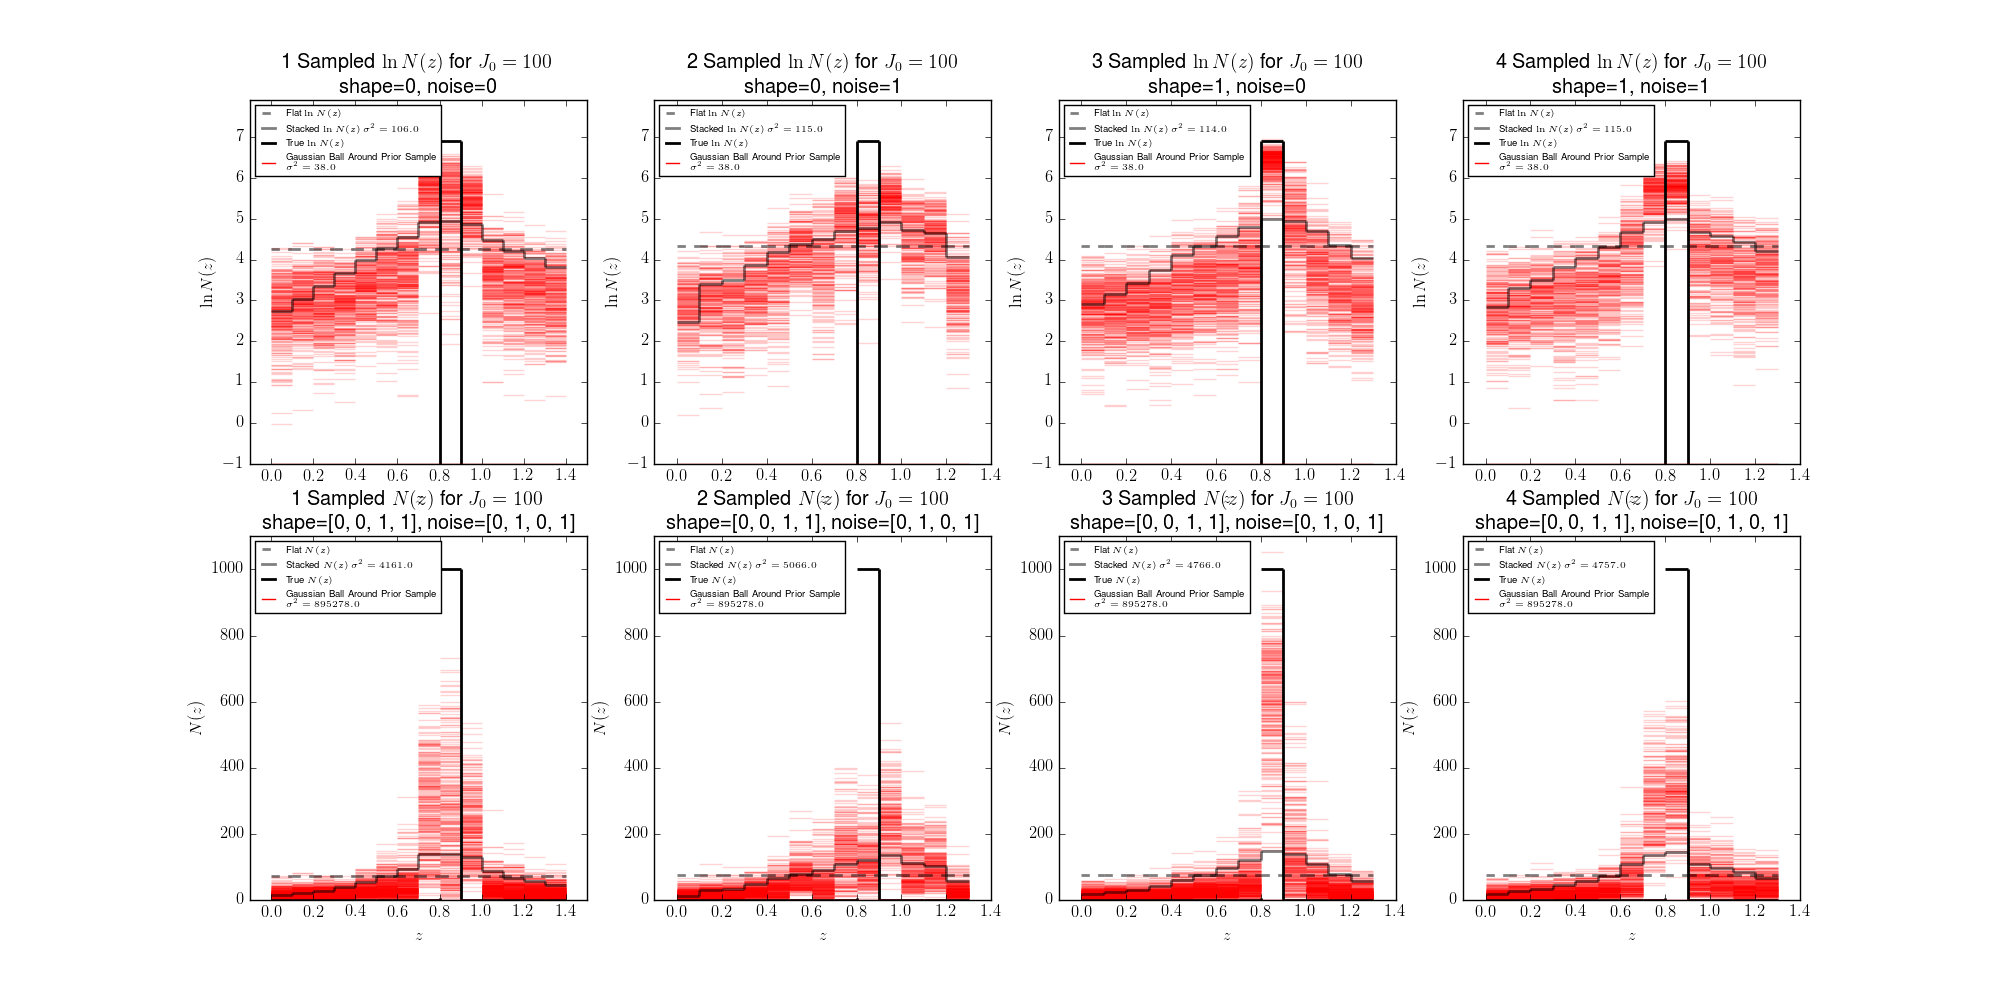
\includegraphics[width=0.5\textwidth]{samps-toy.png}
\caption{The results of the simulation may be seen here.  By way of the $\chi^{2}$ relative to the true value, one can see that in estimating $N(z)$, the result of the stacking method is inferior to the method presented in this paper.}
\label{fig:dumbestparam}
\end{figure}

%The posterior for the entire dataset introduced in Eq. \ref{eq:cancel} may be re-expressed as Eq. \ref{eq:fullpost} in terms of the $K$ bins.  It is valuable to verify that the posterior is maximized for the true $N(z)$ that generated a particular set of simulated data.

%\begin{eqnarray}
%\label{eq:fullpost}
%p(\vec{\theta}|\{\vec{d}_{j}\}_{J}) &=& \frac{p(\vec{\theta})}{p(\{\vec{d}_{j}\}_{J})}\ \exp\left[-\sum_{k=1}^{K}\exp[\theta_{k}]\Delta_{k}\right]\ \prod_{j=1}^{J}\ \sum_{k=1}^{K}\ p(B_{k}|\vec{d}_{j})\ \frac{\exp[\theta_{k}]}{\exp[\theta_{k}^{0}]}\Delta_{k}
%\end{eqnarray}

\clearpage
\subsection{Inappropriate Interim Prior}
\label{sec:interim}

In this case, we vary the interim prior used in the calculation of individual posteriors to show that an inappropriate choice makes a difference in the results.  Typically, zPDFs are made with an interim prior derived from $N(z)$ in a previous observational study.  Since most observational studies used for this purpose are spectroscopically confirmed and objects for which photo-zs are relied upon make up a population that cannot be spectroscopically confirmed, such an interim prior is rarely appropriate.  Some efforts have been made to modify an observationally informed interim prior so that it is more representative of the data set.  \citep{she11}  However, any interim prior of this kind imparts information into the zPDFs and thus the zPDFs.  Ideally, an uninformative interim prior would be used, although it may be complicated to compute from the covariances of the raw data.  In this test, we consider an obviously inappropriate interim prior and compare it to the flat interim prior used in previous tests.

The true $N(z)$ and zPDFs are generated as in Sec. \ref{sec:null} (Fig. \ref{fig:nulltrueNz}), however, the nontrivial interim prior affects the zPDFs and initialization.  

\clearpage
\section{Discussion}
\label{sec:disc}

This study demonstrates a mathematically consistent implementation of inference of a one-point statistic based on zPDFs.  This work supports the production of zPDFs by upcoming photometric surveys such as LSST so that more accurate inference of physical parameters may be accessible to the scientific community.  We discourage researchers from co-adding zPDFs or converting them into point estimates of redshift and instead recommend the use of Bayesian probability to guide the usage of zPDFs in science.

The method herein developed is applicable with minimal modification to other one-point statistics of redshift to which we will apply this method in the future.  Such statistics include the redshift-dependent luminosity function and weak lensing mean distance ratio, the former of which is presented below in Sec. \ref{sec:lf}.

\clearpage
\subsection{The Luminosity Function}
\label{sec:lf}

Since the redshift-dependent luminosity function $\Phi(\vec{L},z)$ is a number density over redshift $z$ and one other parameter, luminosity $\vec{L}$ (which may be a vector if not bolometric), that contributes to the same data $\{\vec{d}_{j}\}_{J}$ in the form of a vector of photometric magnitudes, it is essentially a generalization of the redshift distribution function $N(z)$ previously investigated here; in other words, $N(z)$ is related to $\Phi(\vec{L},z)$ by way of an integral over luminosity.   We may express this as Eq. \ref{eq:lf}, where $\Phi(\vec{L},z)$ is parametrized by hyperparameters that are components of $\vec{\phi}$ .

\begin{eqnarray}
\label{eq:lf}
p(z_{j},\vec{L}_{j}|\vec{\phi}) &=& \frac{\Phi(\vec{L},z)}{\iint \Phi(\vec{L},z)\ d\vec{L}\ dz} = \frac{\Phi(\vec{L},z)}{\int N(z)\ dz} = \frac{1}{J}\ \Phi(\vec{L},z)
\end{eqnarray}

A graphical model for this problem is presented in Fig. \ref{fig:lf}.  As in Sec. \ref{sec:meth}, we shall outline the translation of this graphical representation of the probabilistic model using the same formalism.

\begin{figure}
\vspace{0.5cm}
\begin{center}
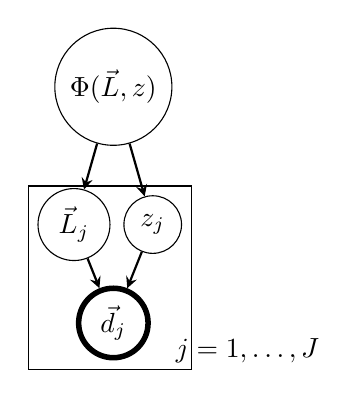
\begin{tikzpicture}[node distance=1cm]

\node (lf) [hyper] {$\Phi(\vec{L},z)$};
\node (z) [param, below of=lf,yshift=-0.75cm,xshift=0.5cm] {$z_{j}$};
\node (L) [param, below of=lf,yshift=-0.75cm,xshift=-0.5cm] {$\vec{L}_{j}$};
\node (flux) [data, below of=lf,yshift=-2cm] {$\vec{d}_{j}$};
\node (survey) [draw=black,fit={(L.west)(z.north)(flux.south)(z.east)}] {};
\node [xshift=1.75cm,yshift=0.25cm] at (survey.south) {$j=1,\dots,J$};

\draw [arrow] (lf) -- (z);
\draw [arrow] (lf) -- (L);
\draw [arrow] (z) -- (flux);
\draw [arrow] (L) -- (flux);

\end{tikzpicture}
\caption{This directed acyclic graph illustrates a hierarchical model for the luminosity function $\Phi(\vec{L},z)$.}
\label{fig:lf}
\end{center}
\end{figure}

First, we assume independence of the $J$ data points $\vec{d}_{j}$ where $J$ is a Poisson random variable with expected value $J_{0}$.  However, we acknowledge that the measurements are not independent if they are made as part of the same experimental design with shared equipment, not to mention the fact that $\vec{L}_{j}$ and $z_{j}$ are not independent of $\vec{L}_{j'\neq j}$ and $z_{j'\neq j}$ respectively due to the physics summarized by the luminosity function $\Phi(\vec{L},z)$.  However, given the assumption of independence, we may write the full likelihood as Eq. \ref{eq:lfind}.  

\begin{eqnarray}
\label{eq:lfind}
p(\{\vec{d}_{j}\}_{J}|\vec{\phi}) &=& e^{-\iint \Phi(\vec{L},z)\ dL\ dz}\ \prod_{j=1}^{J}\ p(\vec{d}_{j}|\vec{\phi})
\end{eqnarray}

As before, we apply Bayes' Rule to relate the full likelihood to the full posterior in Eq. \ref{eq:lfbayes} and expand out the individual likelihood in terms of the parameters $\{\vec{L}_{j}\}_{J}$ and $\{z_{j}\}_{J}$ in Eq. \ref{eq:lfexpand}.

\begin{eqnarray}
\label{eq:lfbayes}
p(\vec{\phi}|\{\vec{d}_{j}\}_{J}) &=& \frac{p(\vec{\phi})}{p(\{\vec{d}_{j}\}_{J})}e^{-\iint \Phi(\vec{L},z)\ d\vec{L}\ dz}\ \prod_{j=1}^{J}\ p(\vec{d}_{j}|\vec{\phi})
\end{eqnarray}

\begin{eqnarray}
\label{eq:lfexpand}
p(\vec{\phi}|\{\vec{d}_{j}\}_{J}) &=& \frac{p(\vec{\phi})}{p(\{\vec{d}_{j}\}_{J})}e^{-\iint \Phi(\vec{L},z)\ d\vec{L}\ dz}\ \prod_{j=1}^{J}\ \iint\ p(\vec{d}_{j}|z_{j},\vec{L}_{j})\ p(z_{j},\vec{L}_{j}|\vec{\phi}) dz_{j}\ d\vec{L}_{j}
\end{eqnarray}

If we are unable to access the individual likelihoods, as is in general the case, we will repeat the trick of using an interim prior value of hyperparameters $\vec{\phi}^{0}$.  This results in Eq. \ref{eq:lftrick}.

\begin{eqnarray}
\label{eq:lftrick}
p(\vec{\phi}|\{\vec{d}_{j}\}_{J}) &=& \frac{p(\vec{\phi})}{p(\{\vec{d}_{j}\}_{J})}e^{-\iint \Phi(\vec{L},z)\ d\vec{L}\ dz}\ \prod_{j=1}^{J}\ \iint\ p(z_{j},\vec{L}_{j}|\vec{d}_{j},\vec{\phi}^{0})\ \frac{p(z_{j},\vec{L}_{j}|\vec{\phi})}{p(z_{j},\vec{L}_{j}|\vec{\phi}^{0})} dz_{j}\ d\vec{L}_{j}
\end{eqnarray}

%Fig. \ref{fig:sheldon} compares the result of summing the posteriors as in Eq. \ref{eq:sheldon} with the result of the MCMC solutions of Eq. \ref{eq:bayes}.  The method of \citet{she11} underestimates the probability of observing low redshifts.  As one would expect, the MCMC estimate irreversibly loses some substructure because of the shifting error added to the simulated data.

%\begin{figure}
%\label{fig:sheldon}
%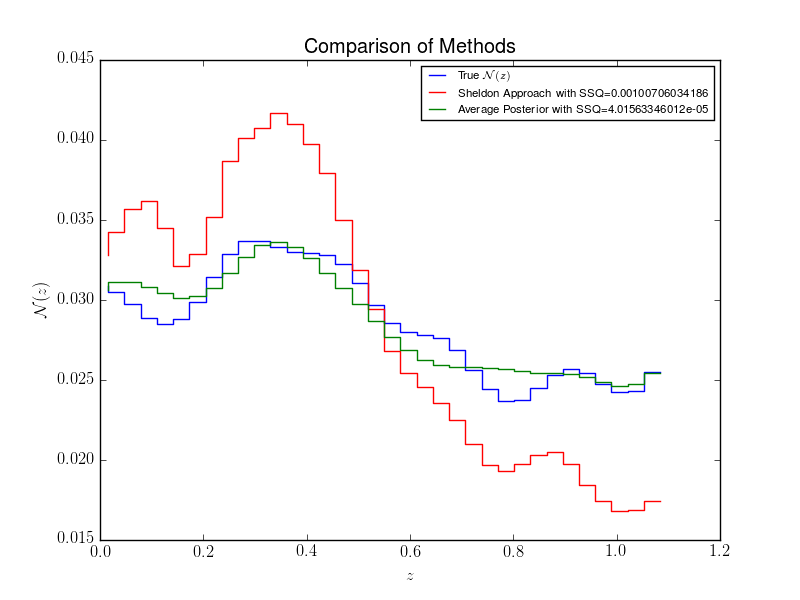
\includegraphics[width=\textwidth]{compare-sheldon.png}
%\caption{The result of applying Eq. \ref{eq:sheldon} is shown in red, the average accepted posterior sample from the method presented here is shown in blue, and $p(z)$ for the observable redshifts of Eq. \ref{eq:zshift} is shown in black.  The sum of squared differences between the result of each method and the true value are also shown; one can see that the \citet{she11} approach has larger errors.}
%\end{figure}

%\acknowledgments

%\subsubsection{}
%\label{app:dumber}

%We next consider a set of $J$ galaxies representing a draw from the Poisson distribution $P(J_{0},J_{0})$ for $J_{0}=100$.  The galaxies share a single true redshift $z^{s}$ arbitrarily chosen to be the midpoint of the redshift bin with the largest $\theta_{k}$.  The redshift posteriors are taken to be single Gaussians centered at observed redshifts $z^{p}_{j}\sim N(z^{s},\bar{\Delta}(1+z^{s}))$ with shared variances of $\bar{\Delta}(1+z^{s})$. 

%\subsubsection{}
%\label{app:dumb}

%The last test case is comprised of a set of $J$ galaxies representing a draw from the Poisson distribution $P(J_{0},J_{0})$ for $J_{0}=1000$.  The true galaxy redshift bins $b_{j}=k$ from $k=1,\dots,K$ are assigned to each galaxy $j$ by randomly sampling the $K$ bins with weights given by the true redshift function of Eq. \ref{eq:truenz} as $\int_{z_{k}}^{z_{k+1}}p^{0}(z)dz$. True redshifts $z^{s}_{j}$ are assigned within these bins assuming a random uniform distribution within each bin.  The redshift posteriors are taken to be single Gaussians centered at observed redshifts $z^{p}_{j}\sim N(z^{s}_{j},\bar{\Delta}(1+z^{s}_{j}))$ with variances $\sigma_{j}\sim N(z^{s}_{j},\bar{\Delta}(1+z^{s}_{j}))$. 

\bibliographystyle{apj}
\bibliography{references}

\end{document}